\documentclass[aspectratio=169,unknownkeysallowed,xcolor=dvipsnames,beamer]{beamer} %handout,notes=show

\usepackage{textcomp}
\usepackage[utf8]{inputenc}
% Locate graphics where you want
\usepackage[absolute,overlay]{textpos}
% \usepackage{default}
\usepackage{graphicx}
%  \usepackage[pdftex]{hyperref}
\usepackage{url}
\usepackage{amsmath}

% frames have to be fragile
\newif\ifnotes
% \notestrue

%\notestrue


\ifnotes
%\setbeamertemplate{note page}[plain]
\setbeamertemplate{note page}[compress]
\setbeamerfont{note page}{size=\large}
\setbeameroption{show only notes}
%\setbeameroption{show notes}
\usepackage{pgfpages}
\pgfpagesuselayout{2 on 1}[a4paper,border shrink=5mm]%
\else
%\setbeameroption{hide notes}
\fi
%\notesfalse



% nastaveni TypeWriter
%\usepackage{courier}
%\usepackage{lmodern}
%\renewcommand*\ttdefault{txtt}
\DeclareFontShape{OT1}{cmtt}{bx}{n}{<5><6><7><8><9><10><10.95><12><14.4><17.28><20.74><24.88>cmttb10}{}


% \usepackage{verbatim}
\usepackage[absolute,overlay]{textpos}

\usepackage{listings}
% \usepackage{courier}
\definecolor{grey}{RGB}{70,70,70}
\definecolor{green}{RGB}{0,255,0}
\definecolor{red}{RGB}{202,53,53}
\definecolor{lightGrey}{RGB}{250,250,250}
\definecolor{darkGrey}{RGB}{50,50,50}


\usepackage{color}
\definecolor{lightgray}{rgb}{.9,.9,.9}
\definecolor{darkgray}{rgb}{.4,.4,.4}
\definecolor{purple}{rgb}{0.65, 0.12, 0.82}

 \usetheme{Boadilla}
% \usetheme{Berkeley}
%\usetheme{Goettingen}
% \usetheme{Montpellier}
% \usetheme{Warsaw}
% \usetheme{Madrid}
% \usetheme{Szeged}
% \useoutertheme{infolines}
%\usecolortheme[named=MidnightBlue]{structure}
\usecolortheme[named=OliveGreen]{structure}
%\usecolortheme[named=PineGreen]{structure}
% \setbeamertemplate{navigation symbols}{}




\title[OGRS 2016]
{\vspace{2cm}\\Assessment of spectral properties\\of Apollo 12 landing site}
%\subtitle{Mini-project ATPS}
%\pdforstring{}{}



\author[Chemin, Crawford, Grindrod, Alexander]
{Yann Chemin, Ian Crawford, Peter Grindrod, Louise Alexander}

\institute[]
{
\begin{center}
 \includegraphics[width=2.5cm]{Birkbeck}
\end{center}
}
\date{\tiny \textcolor{white}{April 27$^{th}$, 2016}}


%\AtBeginSection[]{\begin{frame}\frametitle{Obsah}%
%\tableofcontents[currentsection ]\end{frame}}
%\AtBeginSubsection[]
%{
%  \begin{frame}<beamer>
%  \frametitle{Obsah}
%  \tableofcontents[currentsection,currentsubsection]
%  \end{frame}
%}

\setbeamercovered{transparent}

\hypersetup{%
	pdfauthor={Yann Chemin},%
	pdfsubject={BSc project talk: Assessment of spectral properties of Apollo 12 landing site},%
    pdfkeywords={Moon, Chandrayaan-1, M3, CPX, Copernicus ray, hyperspectral, remote sensing, Apollo 12}
}

\usepackage{listings}
\lstdefinestyle{C++}{%
  % language
  language=C++, % [ANSI]C++, GNU, ISO, Visual
  basicstyle=\ttfamily\small,
  commentstyle=\itshape,
  keywordstyle=\bfseries, % needs another \ttdefault
  showstringspaces=false,
  stringstyle=,
  identifierstyle=,
  % working with latex
  escapeinside={//lst}{\^^M}  
}

\lstset{%
%  frame=trBL,
%  backgroundcolor=\color{},
  linewidth=\textwidth,
  % working with latex
  gobble=2,
  % float
  nolol=false,
  numberbychapter=true,
  captionpos=t,% tb
  % breaking lines
  breaklines=true,
  breakatwhitespace=true,
  breakindent=10em,
  breakautoindent=true,
  prebreak={},
  postbreak={},
  %document default style
    basicstyle=\ttfamily
}


%\lstlistlistingname % The header name for the list of listings.
%\lstlistingname % The caption label for listings.

\lstnewenvironment{cmdline}[1][]
{\lstset{
  style=C++,
  #1}}
{}

\lstnewenvironment{scpp}[1][]
{\lstset{
  style=C++,
  #1}}
{}

\lstnewenvironment{ncpp}[1][]
{\lstset{
  style=C++,
  numbers=left, 
  numberstyle=\scriptsize, 
  stepnumber=1,
  numbersep=5pt,
  #1}}
{}

\lstnewenvironment{fcpp}[1][]
{\lstset{
  style=C++,
  float,
   % line numbers
  numbers=left, 
  numberstyle=\scriptsize, 
  stepnumber=1,
  numbersep=5pt,
  #1}}
{}


\lstnewenvironment{lcpp}[1][]
{\lstset{%
style=C++,
numbers=left, 
numberstyle=\scriptsize, 
stepnumber=1,
numbersep=5pt,
xleftmargin=12pt,
breakautoindent=false,
breaklines=false,%
#1}}{}

\lstnewenvironment{smallcpp}[1][]
{\lstset{%
style=C++,
numbers=left, 
numberstyle=\tiny, 
stepnumber=1,
numbersep=5pt,
xleftmargin=12pt,
breakautoindent=false,
breaklines=false,%
basicstyle=\ttfamily\scriptsize,
#1}}{}


\lstnewenvironment{pscpp}[1][]
{\lstset{%
style=C++,
xleftmargin=12pt,
breakautoindent=false,
breaklines=false,
#1}}{}


%\lstset{index={square},index={[2]root}}


\newcommand{\overovaciref}[1]{{\scriptsize(\ref{#1})}}


\usepackage{tipa}
\newcommand{\pron}[2]{#1 [#2]}

%%%%%%%%%%%%%%%%%%%%%%%%%%%%%%%%%%%%%%%%%%%%%%%%%%%%%%%%%%%%%%%%%%%%
% TOC frame setup
%%%%%%%%%%%%%%%%%%%%%%%%%%%%%%%%%%%%%%%%%%%%%%%%%%%%%%%%%%%%%%%%%%%%
\usepackage{multicol}
\colorlet{mycolor}{orange!80!black}% change this color to suit your needs
\AtBeginSection[]{
  \setbeamercolor{section in toc shaded}{use=structure,fg=structure.fg}
  \setbeamercolor{section in toc}{fg=mycolor}
  \setbeamercolor{subsection in toc shaded}{fg=black}
  \setbeamercolor{subsection in toc}{fg=mycolor}
  \frame<beamer>{\begin{multicols}{2}
  \frametitle{Outline}
  \setcounter{tocdepth}{2}  
  \tableofcontents[currentsection,subsections]
\end{multicols} 
 }
}

\setbeamercolor{author in head/foot}{fg=white}
\setbeamercolor{title in head/foot}{fg=white}
\setbeamercolor{section in head/foot}{fg=mycolor}
\setbeamertemplate{section in head/foot shaded}{\color{white!70!black}\insertsectionhead}
\setbeamercolor{subsection in head/foot}{fg=mycolor}
\setbeamertemplate{subsection in head/foot shaded}{\color{white!70!black}\insertsubsectionhead}
\setbeamercolor{frametitle}{fg=white}
\setbeamercolor{framesubtitle}{fg=white}

%%%%%%%%%%%%%%%%%%%%%%%%%%%%%%%%%%%%%%%%%%%%%%%%%%%%%%%%%%%%%%%%%%%%
%%%%%%%%%%%%%%%%%%%%%%%%%%%%%%%%%%%%%%%%%%%%%%%%%%%%%%%%%%%%%%%%%%%%
%%%%%%%%%%%%%%%%%%%%%%%%%%%%%%%%%%%%%%%%%%%%%%%%%%%%%%%%%%%%%%%%%%%%
\begin{document}


%%%%%%%%%%%%%%%%%%%%%%%%%%%%%%%%%%%%%%%%%%%%%%%%%%%%%%%%%%%%%%%%%%%%
\begin{frame}
 \maketitle
\end{frame}
%%%%%%%%%%%%%%%%%%%%%%%%%%%%%%%%%%%%%%%%%%%%%%%%%%%%%%%%%%%%%%%%%%%%

%%%%%%%%%%%%%%%%%%%%%%%%%%%%%%%%%%%%%%%%%%%%%%%%%%%%%%%%%%%%%%%%%%%%
\begin{frame}{Contents}
 \begin{multicols}{2}
  \setcounter{tocdepth}{2}  
  \tableofcontents
 \end{multicols} 
\end{frame}
%%%%%%%%%%%%%%%%%%%%%%%%%%%%%%%%%%%%%%%%%%%%%%%%%%%%%%%%%%%%%%%%%%%%

\section{Preamble}
%%%%%%%%%%%%%%%%%%%%%%%%%%%%%%%%%%%%%%%%%%%%%%%%%%%%%%%%%%%%%%%%%%%%
{\usebackgroundtemplate{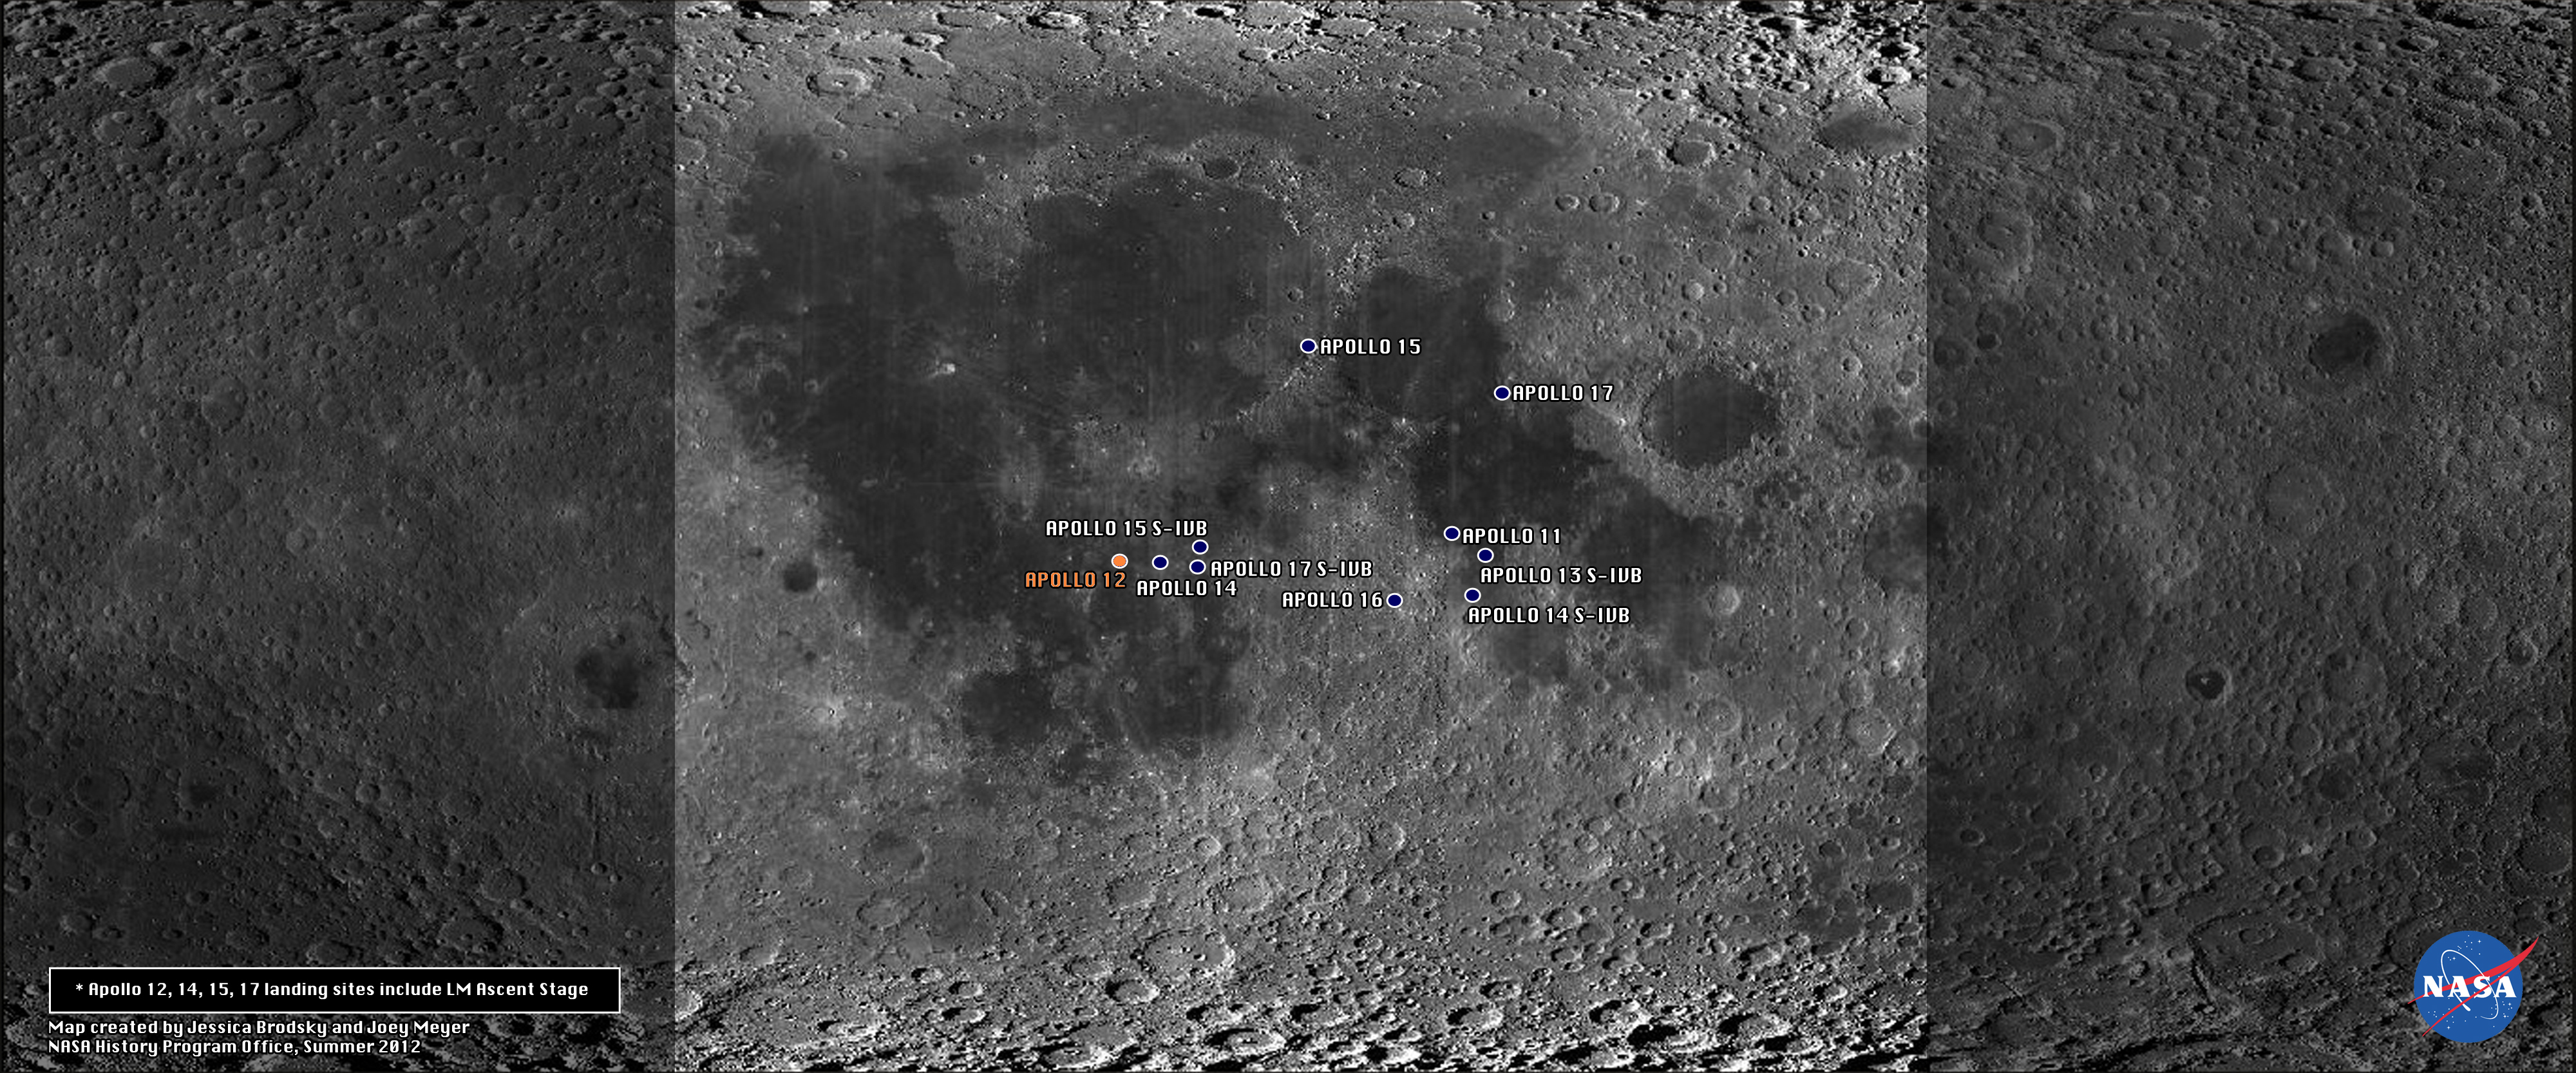
\includegraphics[height=\paperheight,width=\paperwidth]{images/A12_location_map}}
\begin{frame}[plain]
%\begin{center}
  %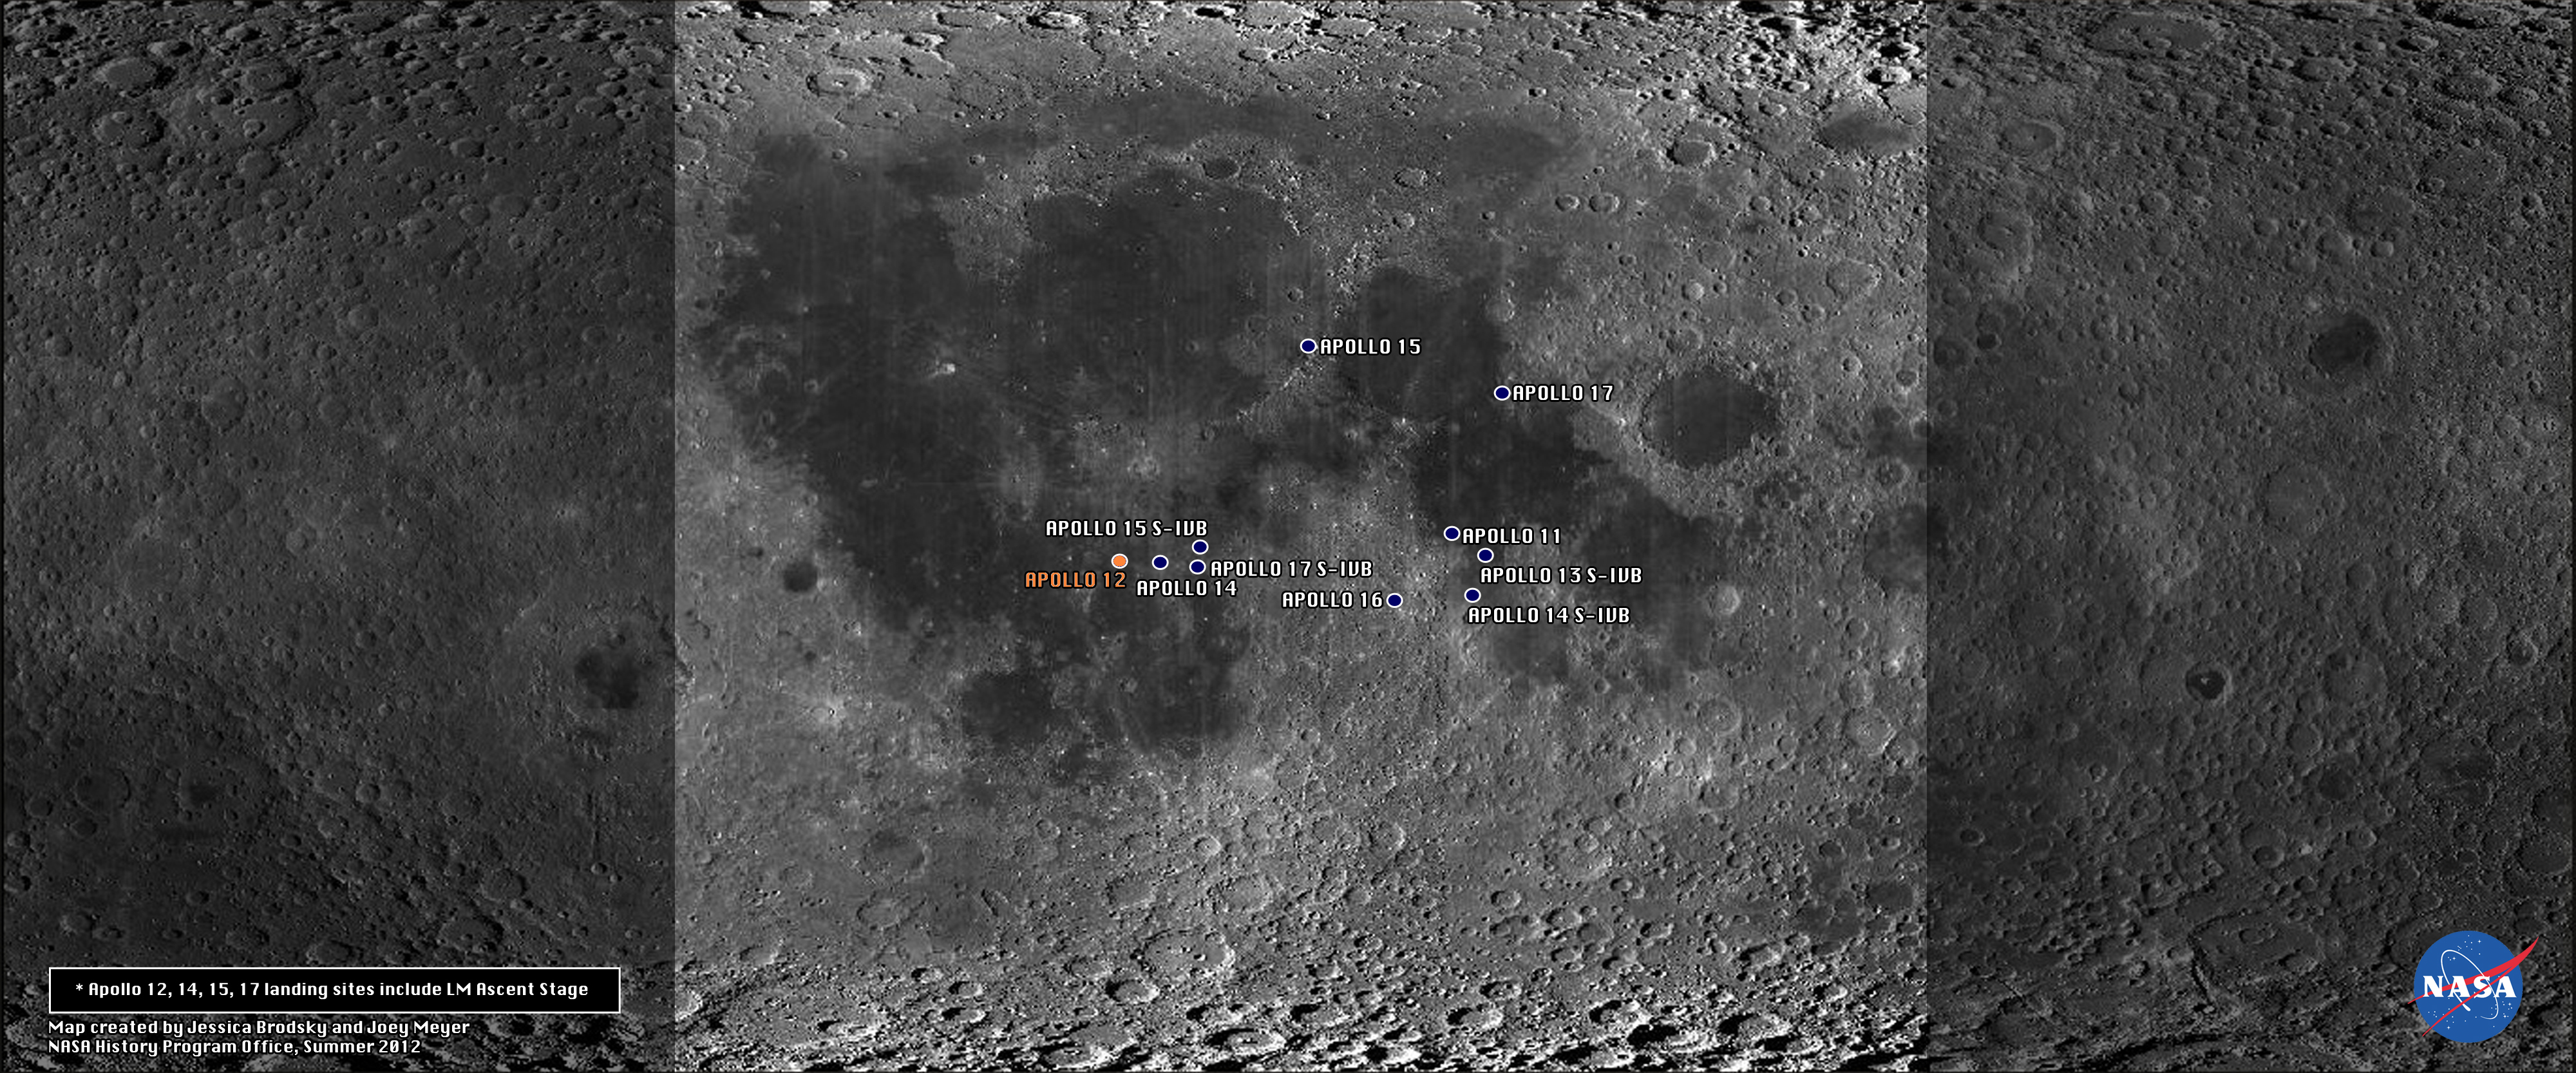
\includegraphics[width=12cm]{images/A12_location_map}
%\end{center}
\end{frame}}
%%%%%%%%%%%%%%%%%%%%%%%%%%%%%%%%%%%%%%%%%%%%%%%%%%%%%%%%%%%%%%%%%%%%
\begin{frame}[fragile]{Preamble1}
\subsection{Location/timelines}
\begin{multicols}{2}
\begin{textblock*}{5cm}(-0.08cm,-0,07cm) % {block width} (coords)
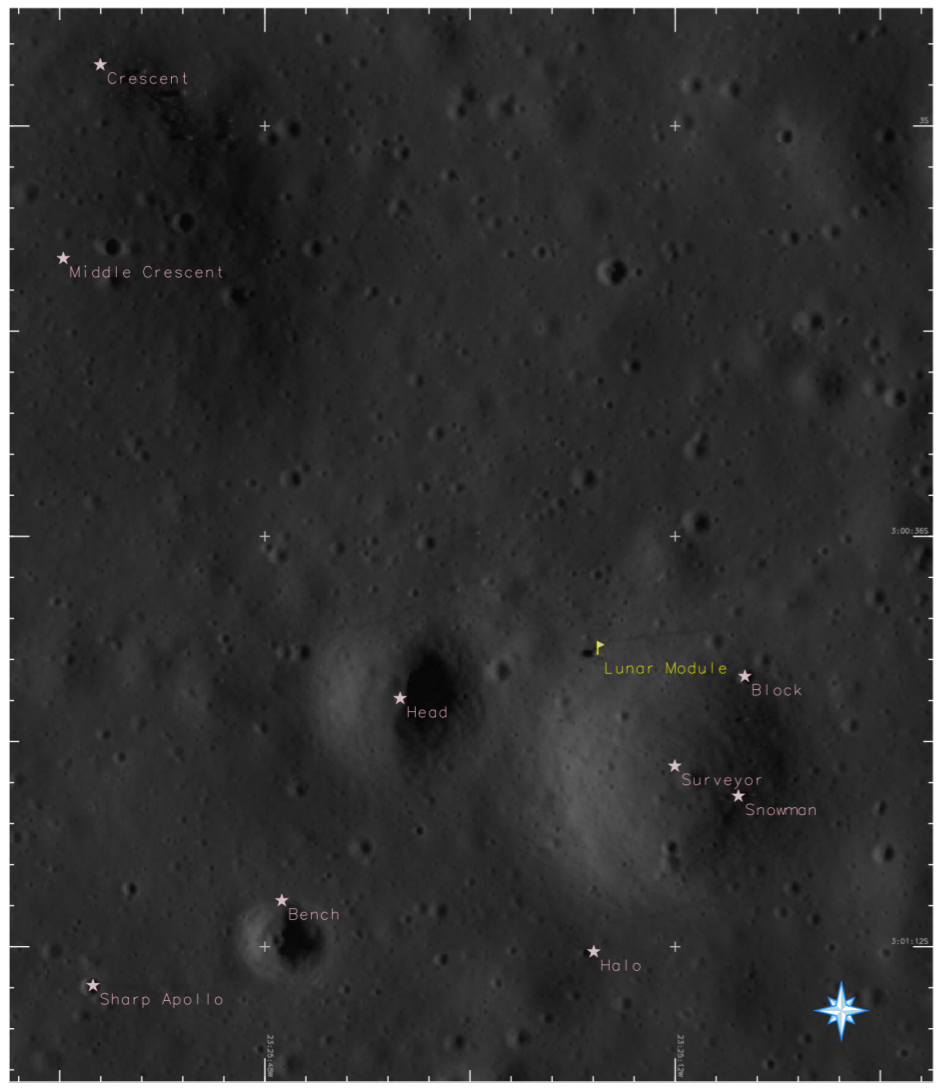
\includegraphics[width=8.08cm]{images/fig1}
\end{textblock*}
\begin{textblock*}{7cm}(8cm,2cm){Location/timelines}
\scriptsize
\begin{itemize}
\item 3.2S 336.62E
\item Surveyor: 19 April 1967
\item Apollo 12: 19 November 1969
\item Chan-1: 2 October, 2008
\item Chan-1: 312 days
\item (LROC NAC image here)
\end{itemize}
\vspace{5mm}
Fortezzo and Hare (2013) classify Apollo 12 landing site in an Erastothenian system with an age ranging from 1.1 to 3.2 Ga.
\end{textblock*}
\end{multicols}
\end{frame}
%%%%%%%%%%%%%%%%%%%%%%%%%%%%%%%%%%%%%%%%%%%%%%%%%%%%%%%%%%%%%%%%%%%%
{\usebackgroundtemplate{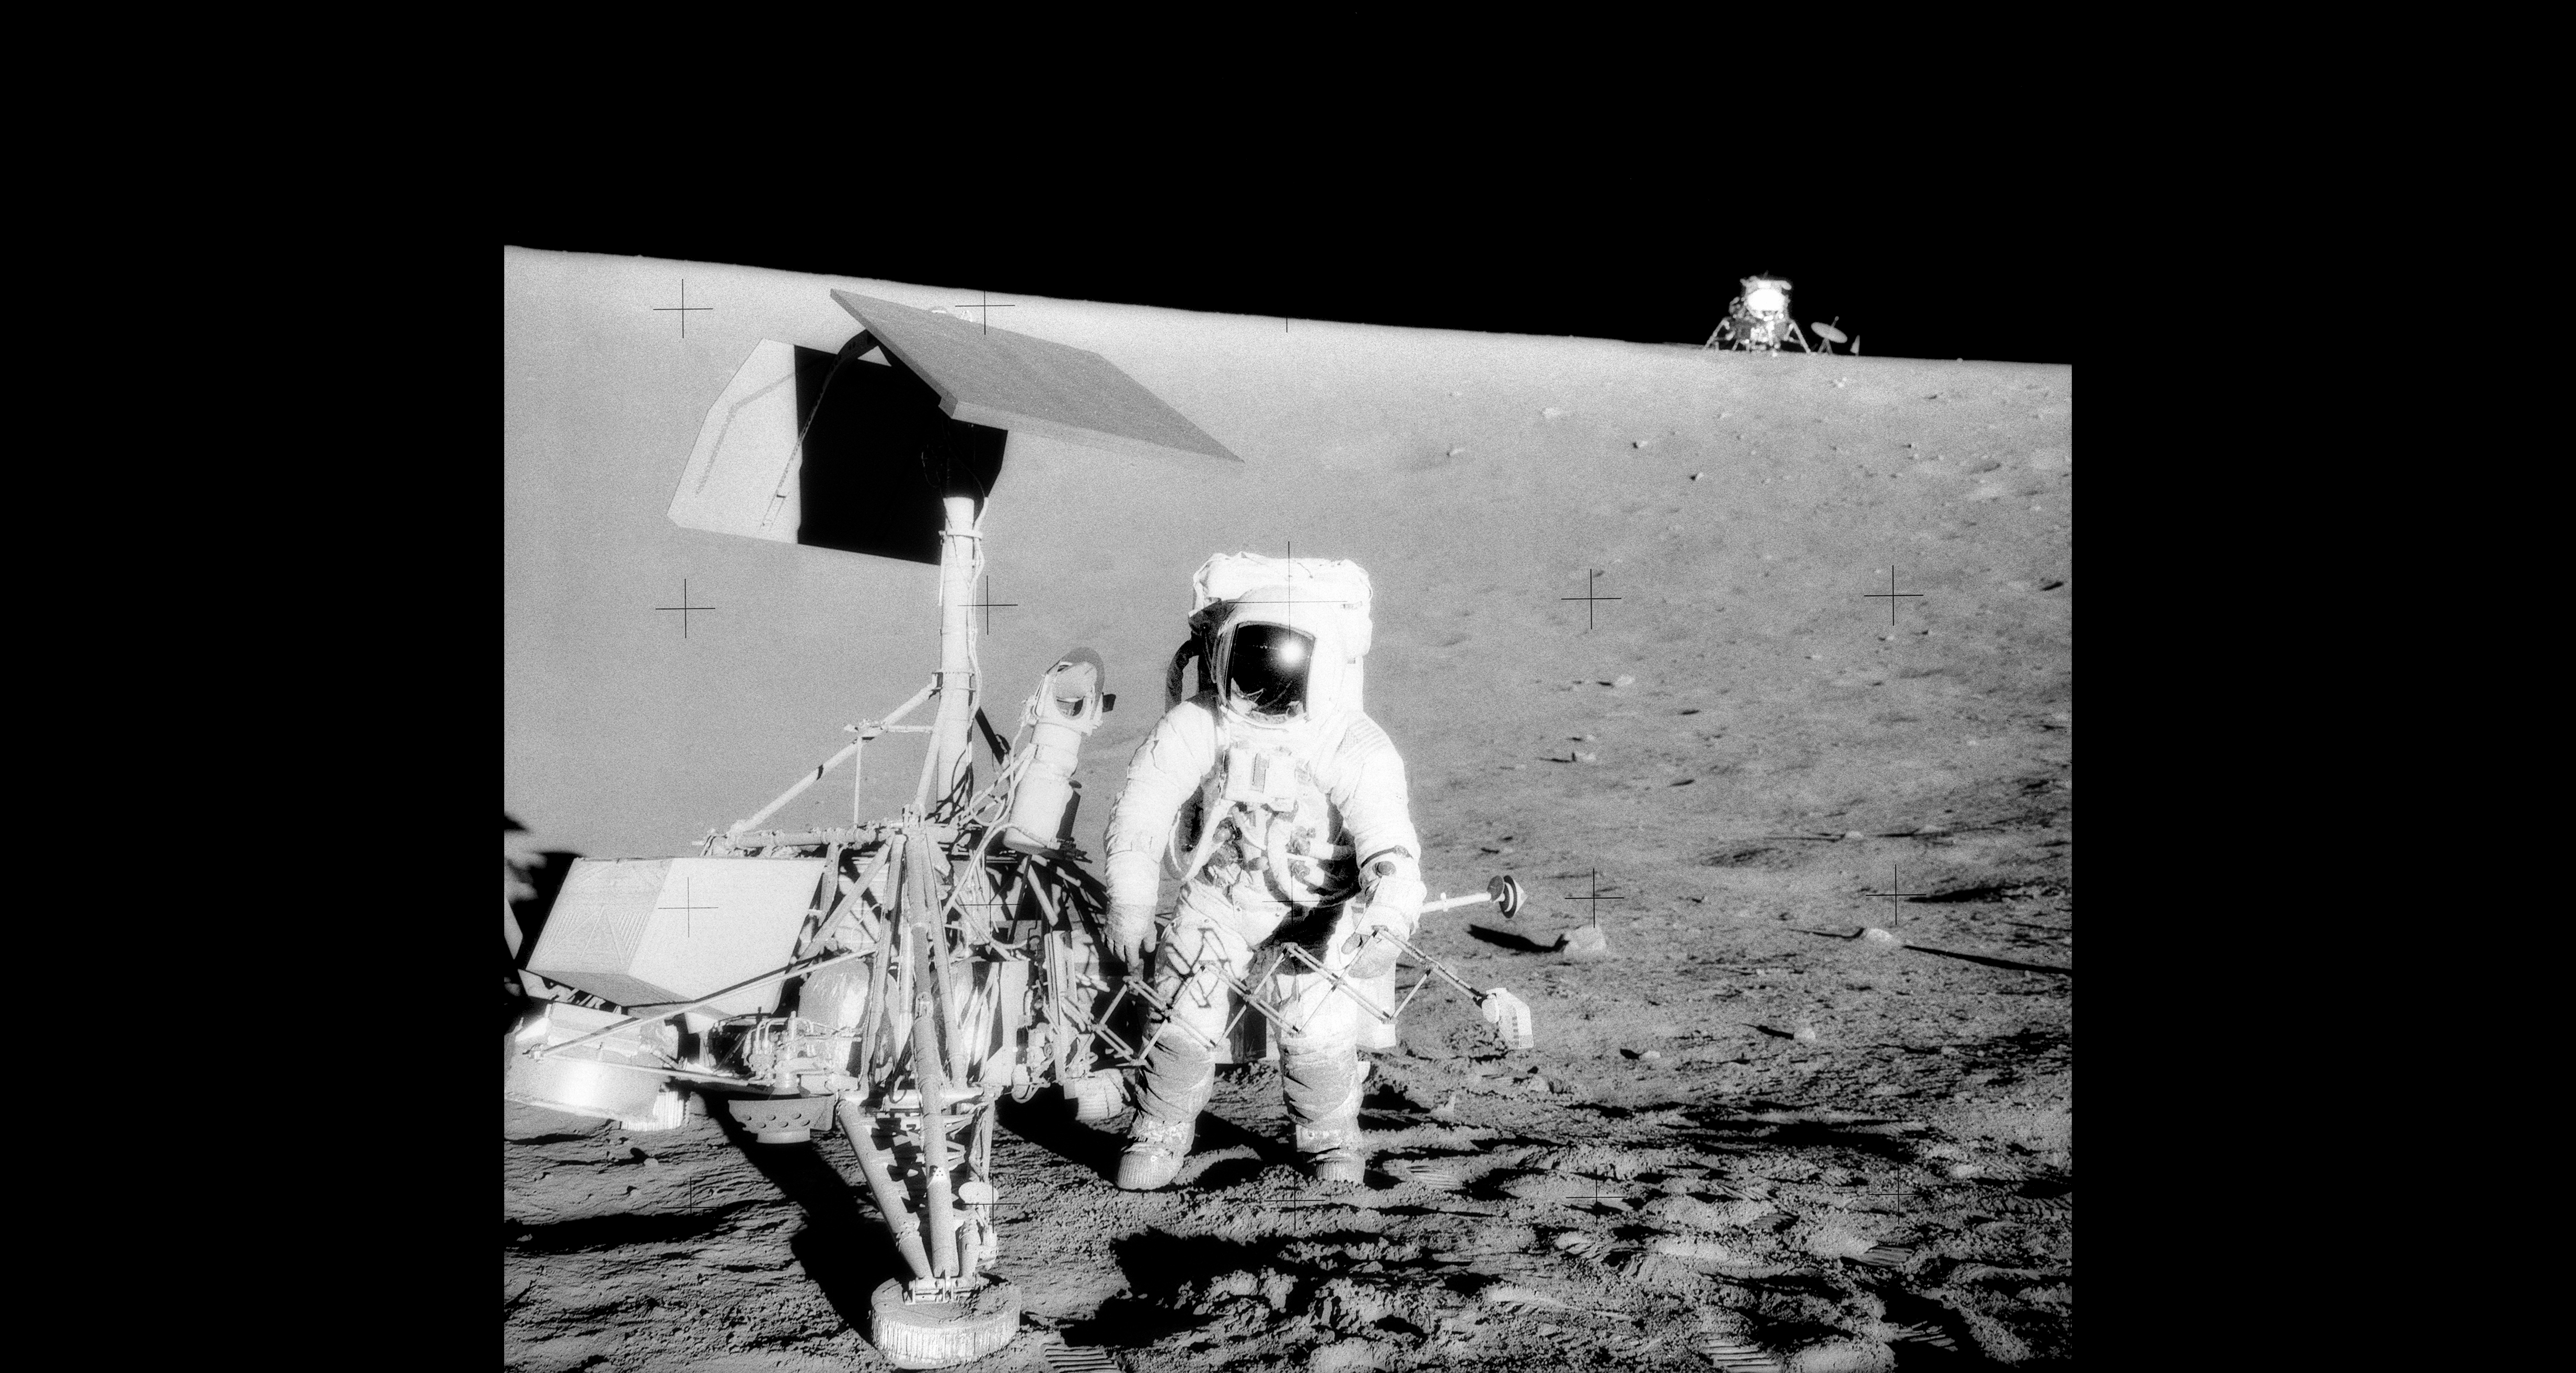
\includegraphics[height=\paperheight,width=\paperwidth]{images/Surveyor_3-Apollo_12}}
\begin{frame}[plain]
%\begin{center}
  %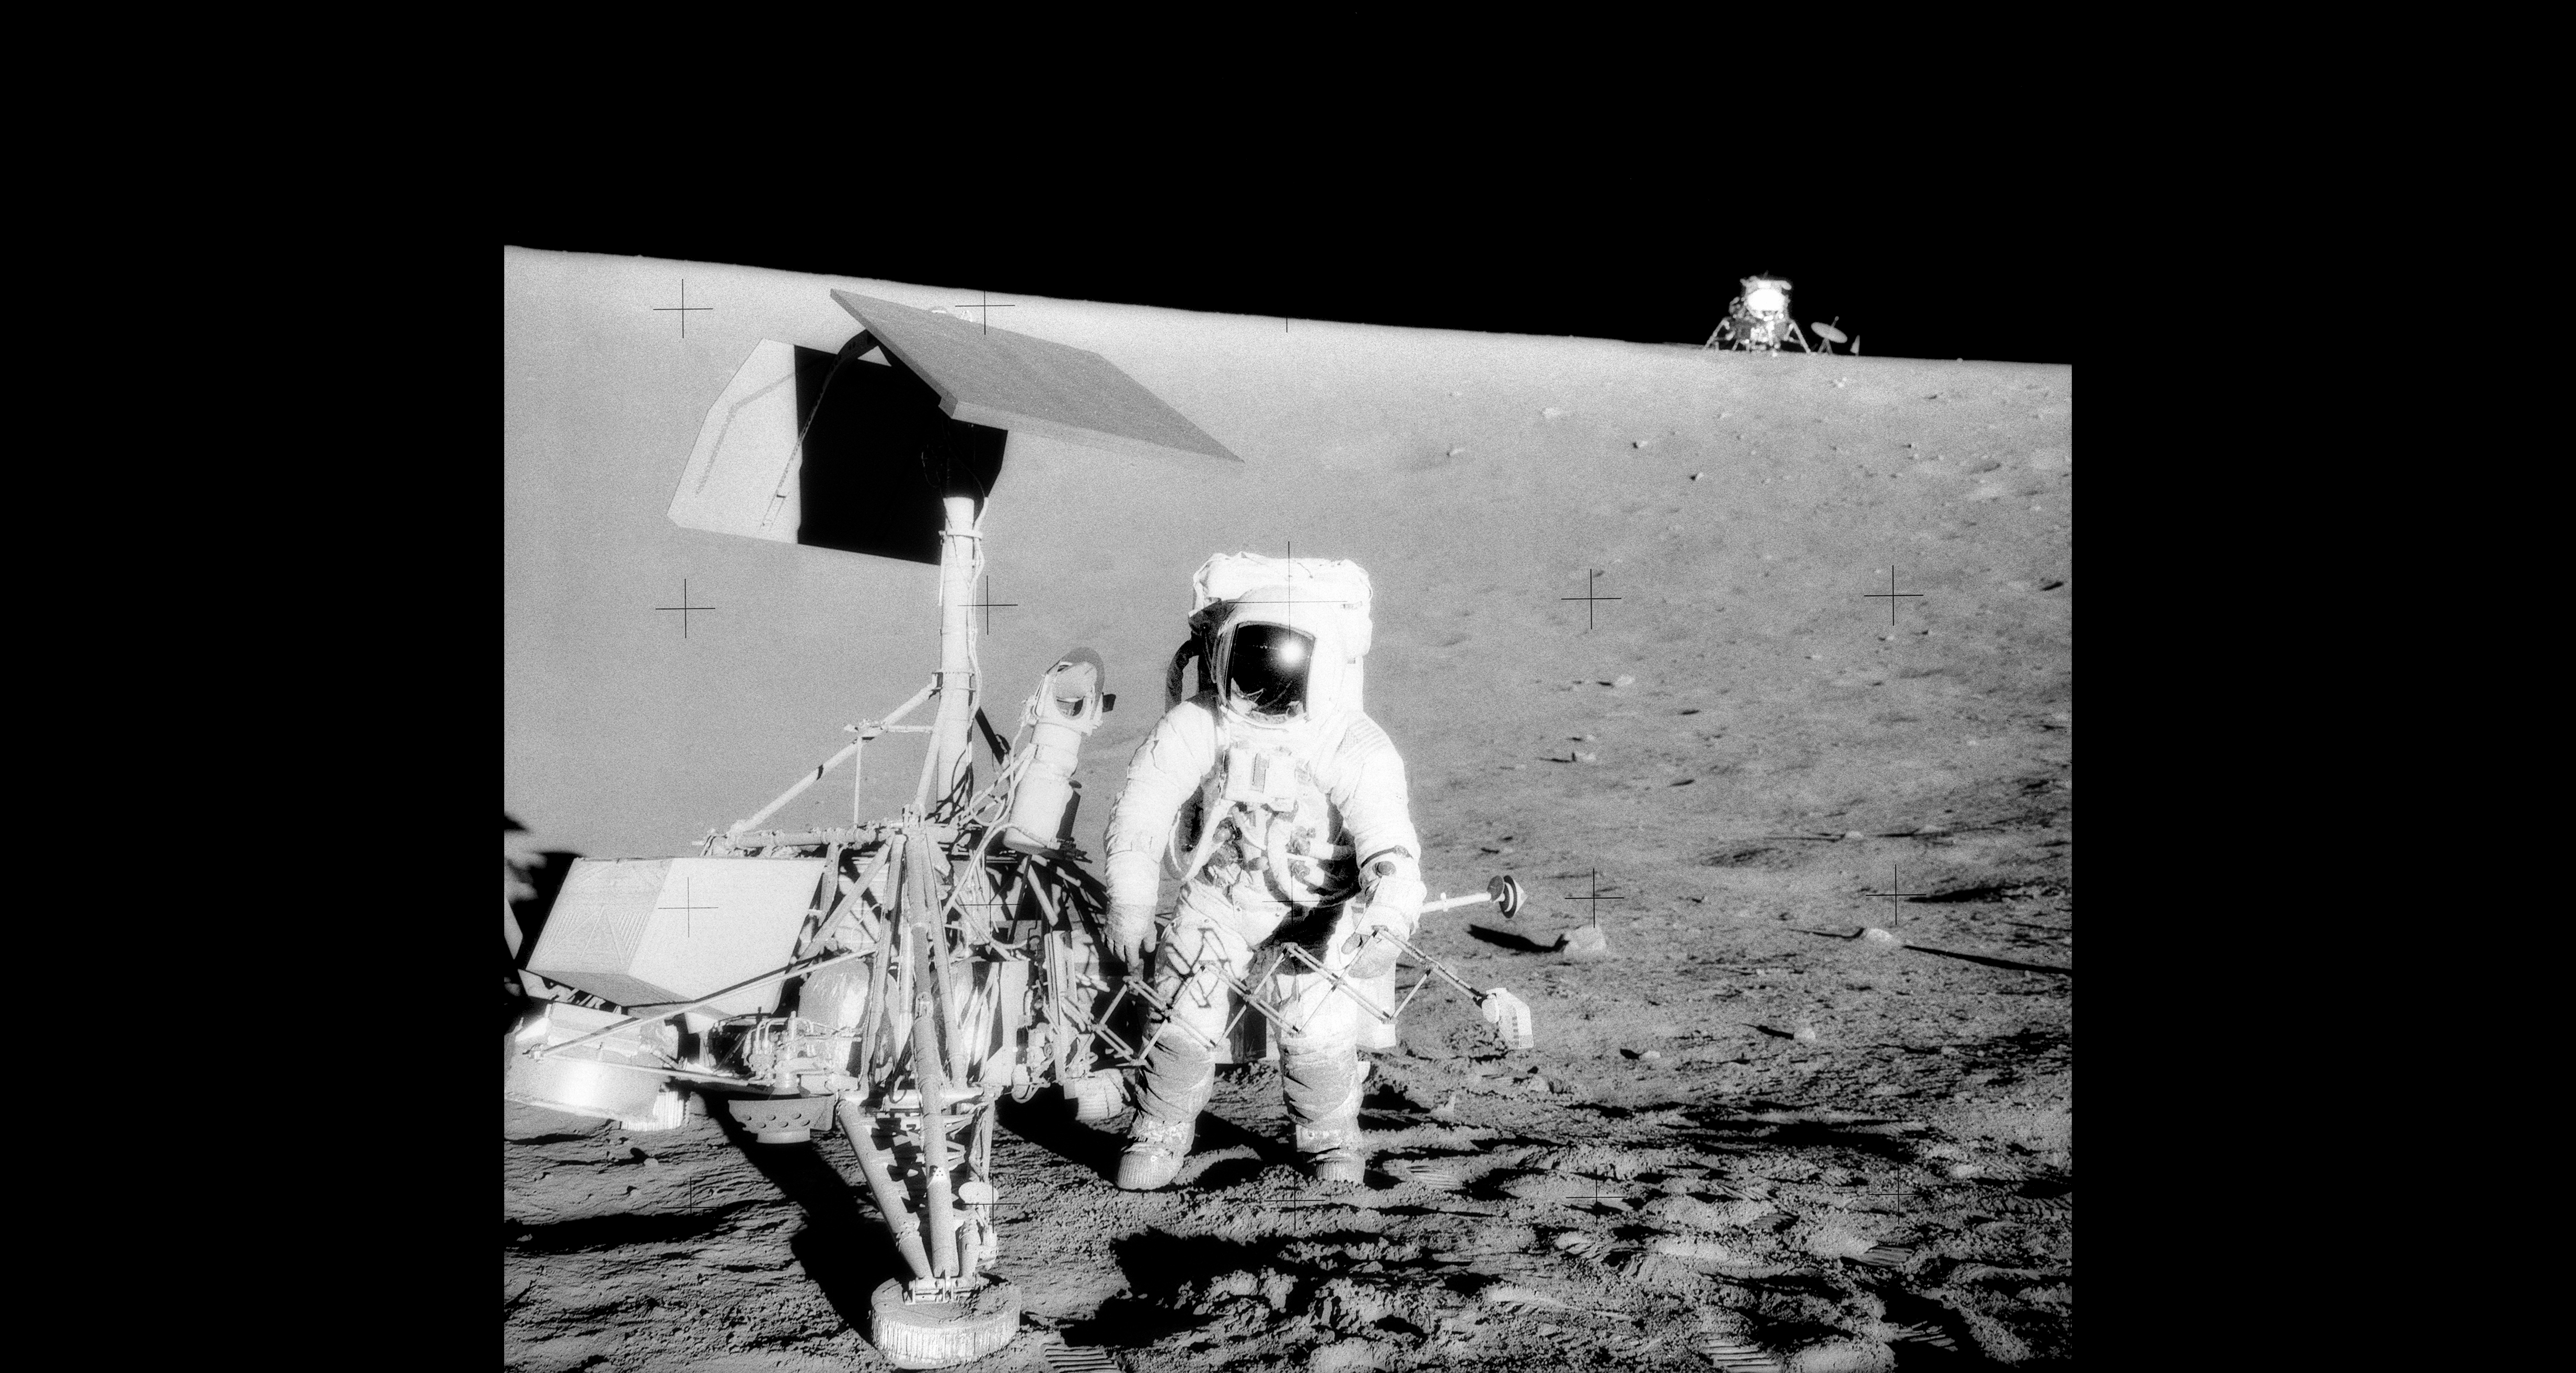
\includegraphics[width=10.5cm]{images/Surveyor_3-Apollo_12}
%\end{center}
\end{frame}}
%%%%%%%%%%%%%%%%%%%%%%%%%%%%%%%%%%%%%%%%%%%%%%%%%%%%%%%%%%%%%%%%%%%%
\begin{frame}[fragile]{Preamble2}
\subsection{Objectives}
\begin{block}{Objectives}
\begin{itemize}
\item Initially designed to complement Alexander [2015]$^*$
\item Different scale and point of view from remote sensing
\item Keeping the scale at the landing site level
\item Using the Moon Multispectral Mapper (M$^3$) @150m/pixel
\end{itemize}
\end{block}
\begin{block}{}
\begin{itemize}
\item Hyperspectral signatures from lunar samples
\item Hyperspectral response curves from M$^3$
\item Can we say something from those about the A12 landing site?
\end{itemize}
\end{block}
[$^*$]{\small Alexander, L. \textit{A geochemical and mineralogical study of lunar basaltic fines collected at the Apollo 12 landing site}. PhD thesis, University of London, London, U.K.,
2015.}
\end{frame}
%%%%%%%%%%%%%%%%%%%%%%%%%%%%%%%%%%%%%%%%%%%%%%%%%%%%%%%%%%%%%%%%%%%%
\begin{frame}[fragile]{Preamble3}
\subsection{Cross-section}
\begin{block}{Cross-section}
\begin{center}
  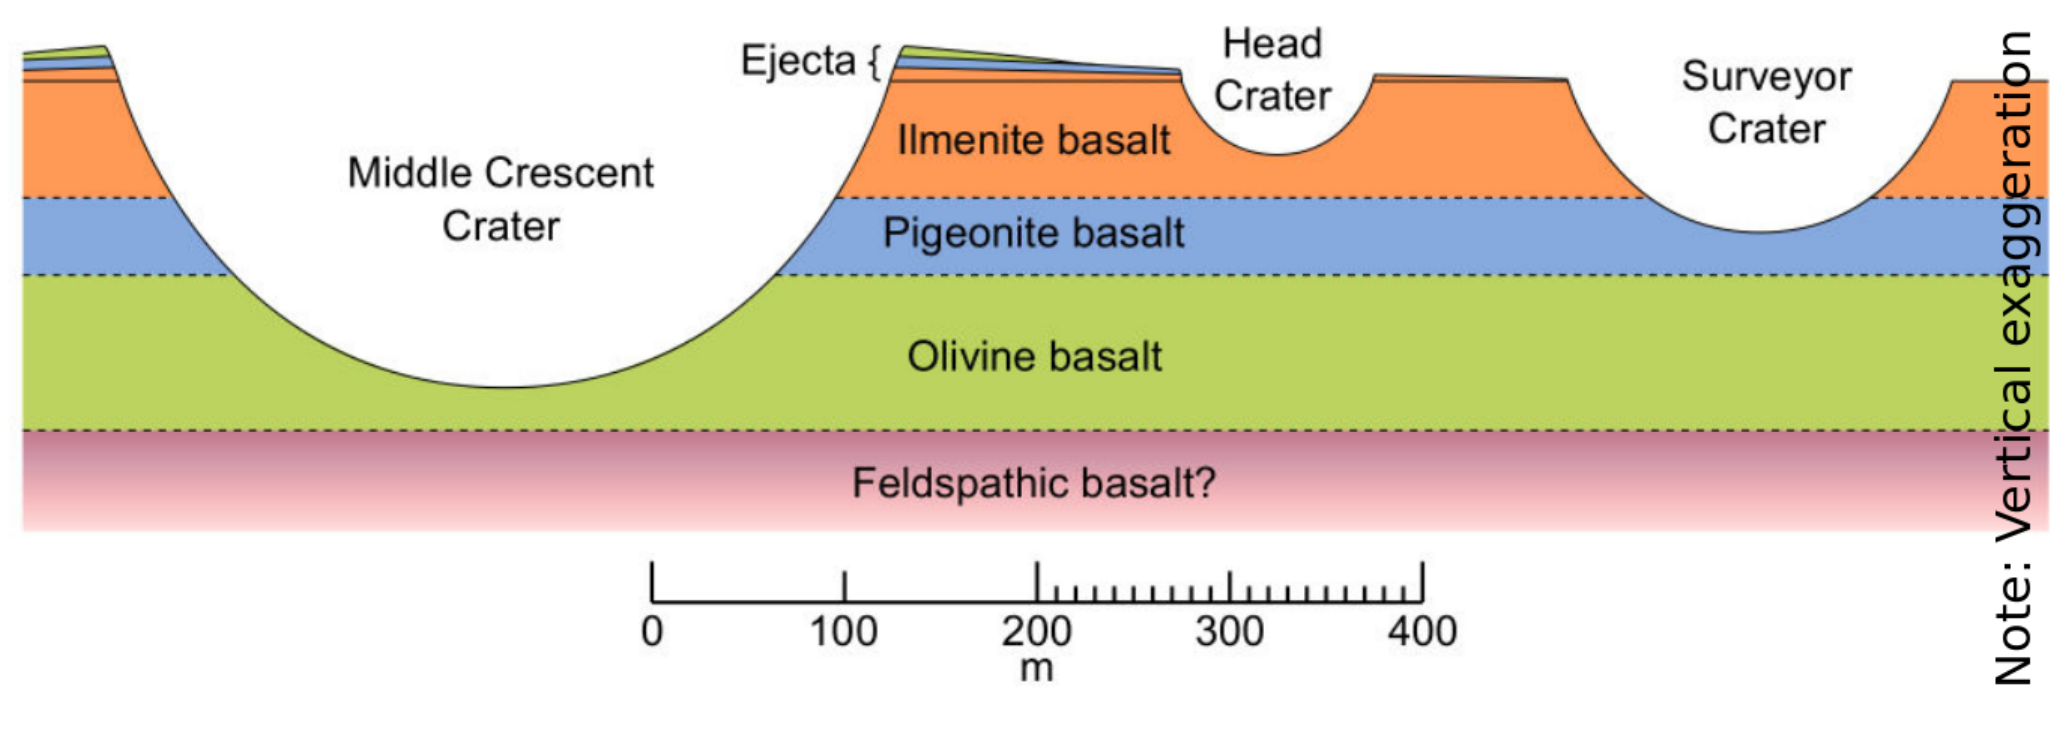
\includegraphics[width=14cm]{images/fig2}\\
  Apollo 12 Landing site mineralogical cross-section [Snape et al., 2013]
\end{center}
\end{block}
\end{frame}

\section{Chandrayaan-1 M$^3$}
%%%%%%%%%%%%%%%%%%%%%%%%%%%%%%%%%%%%%%%%%%%%%%%%%%%%%%%%%%%%%%%%%%%%
{\usebackgroundtemplate{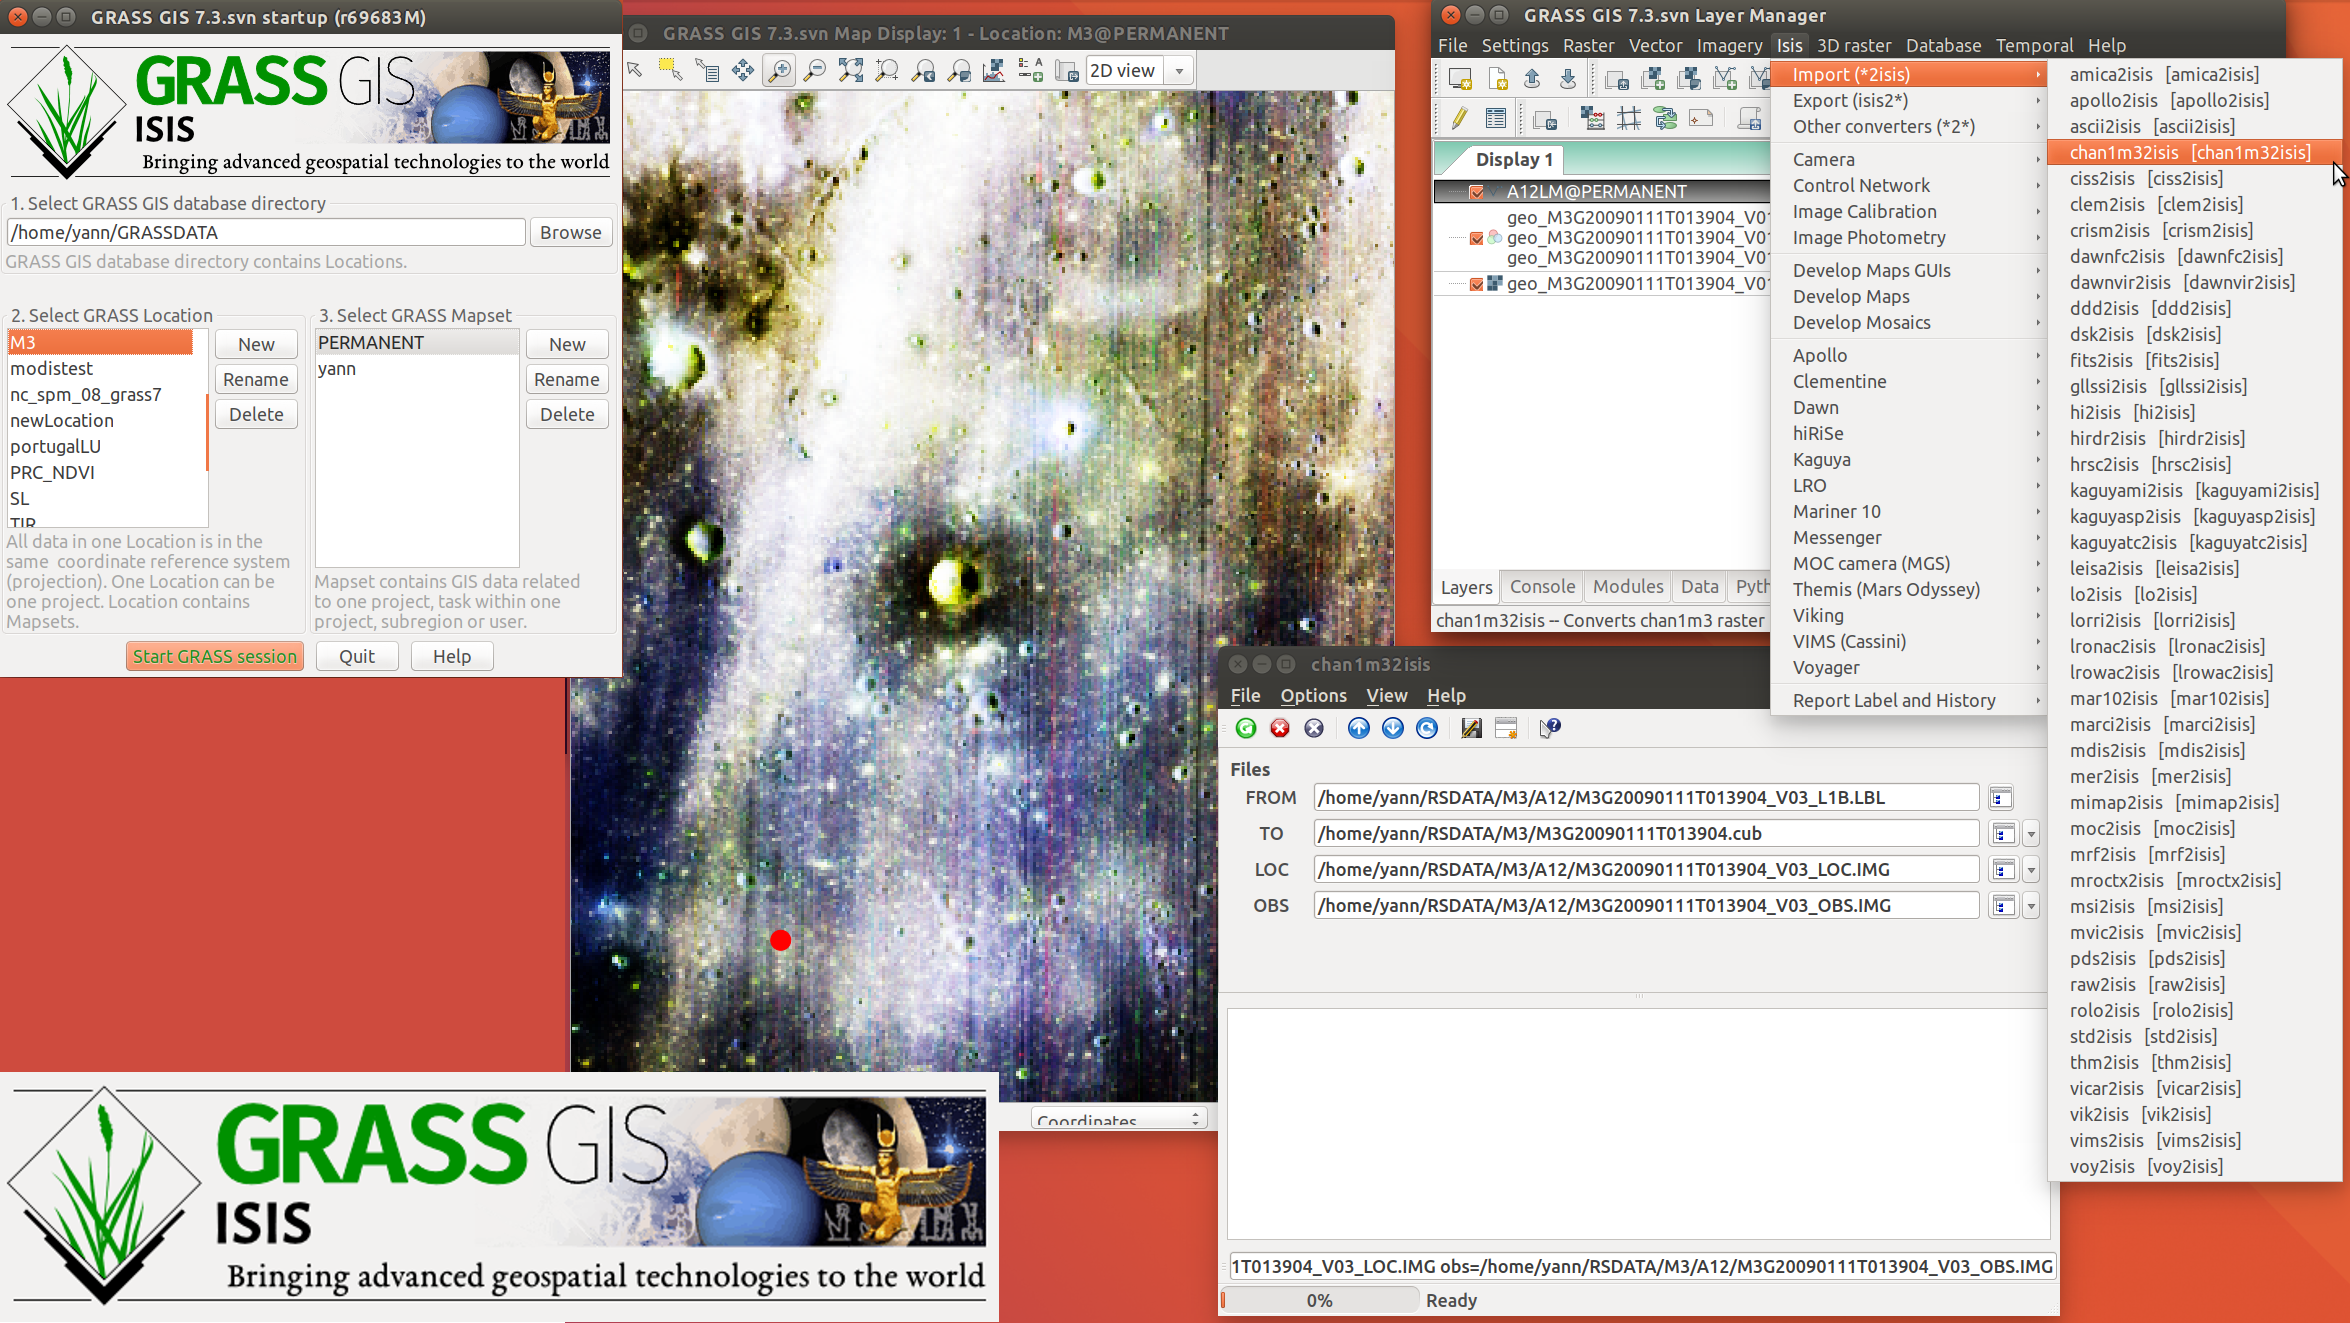
\includegraphics[height=\paperheight,width=\paperwidth]{images/ISISwithGRASS}}
\begin{frame}[plain]
%\subsection{Import data}
%\begin{center}
 % 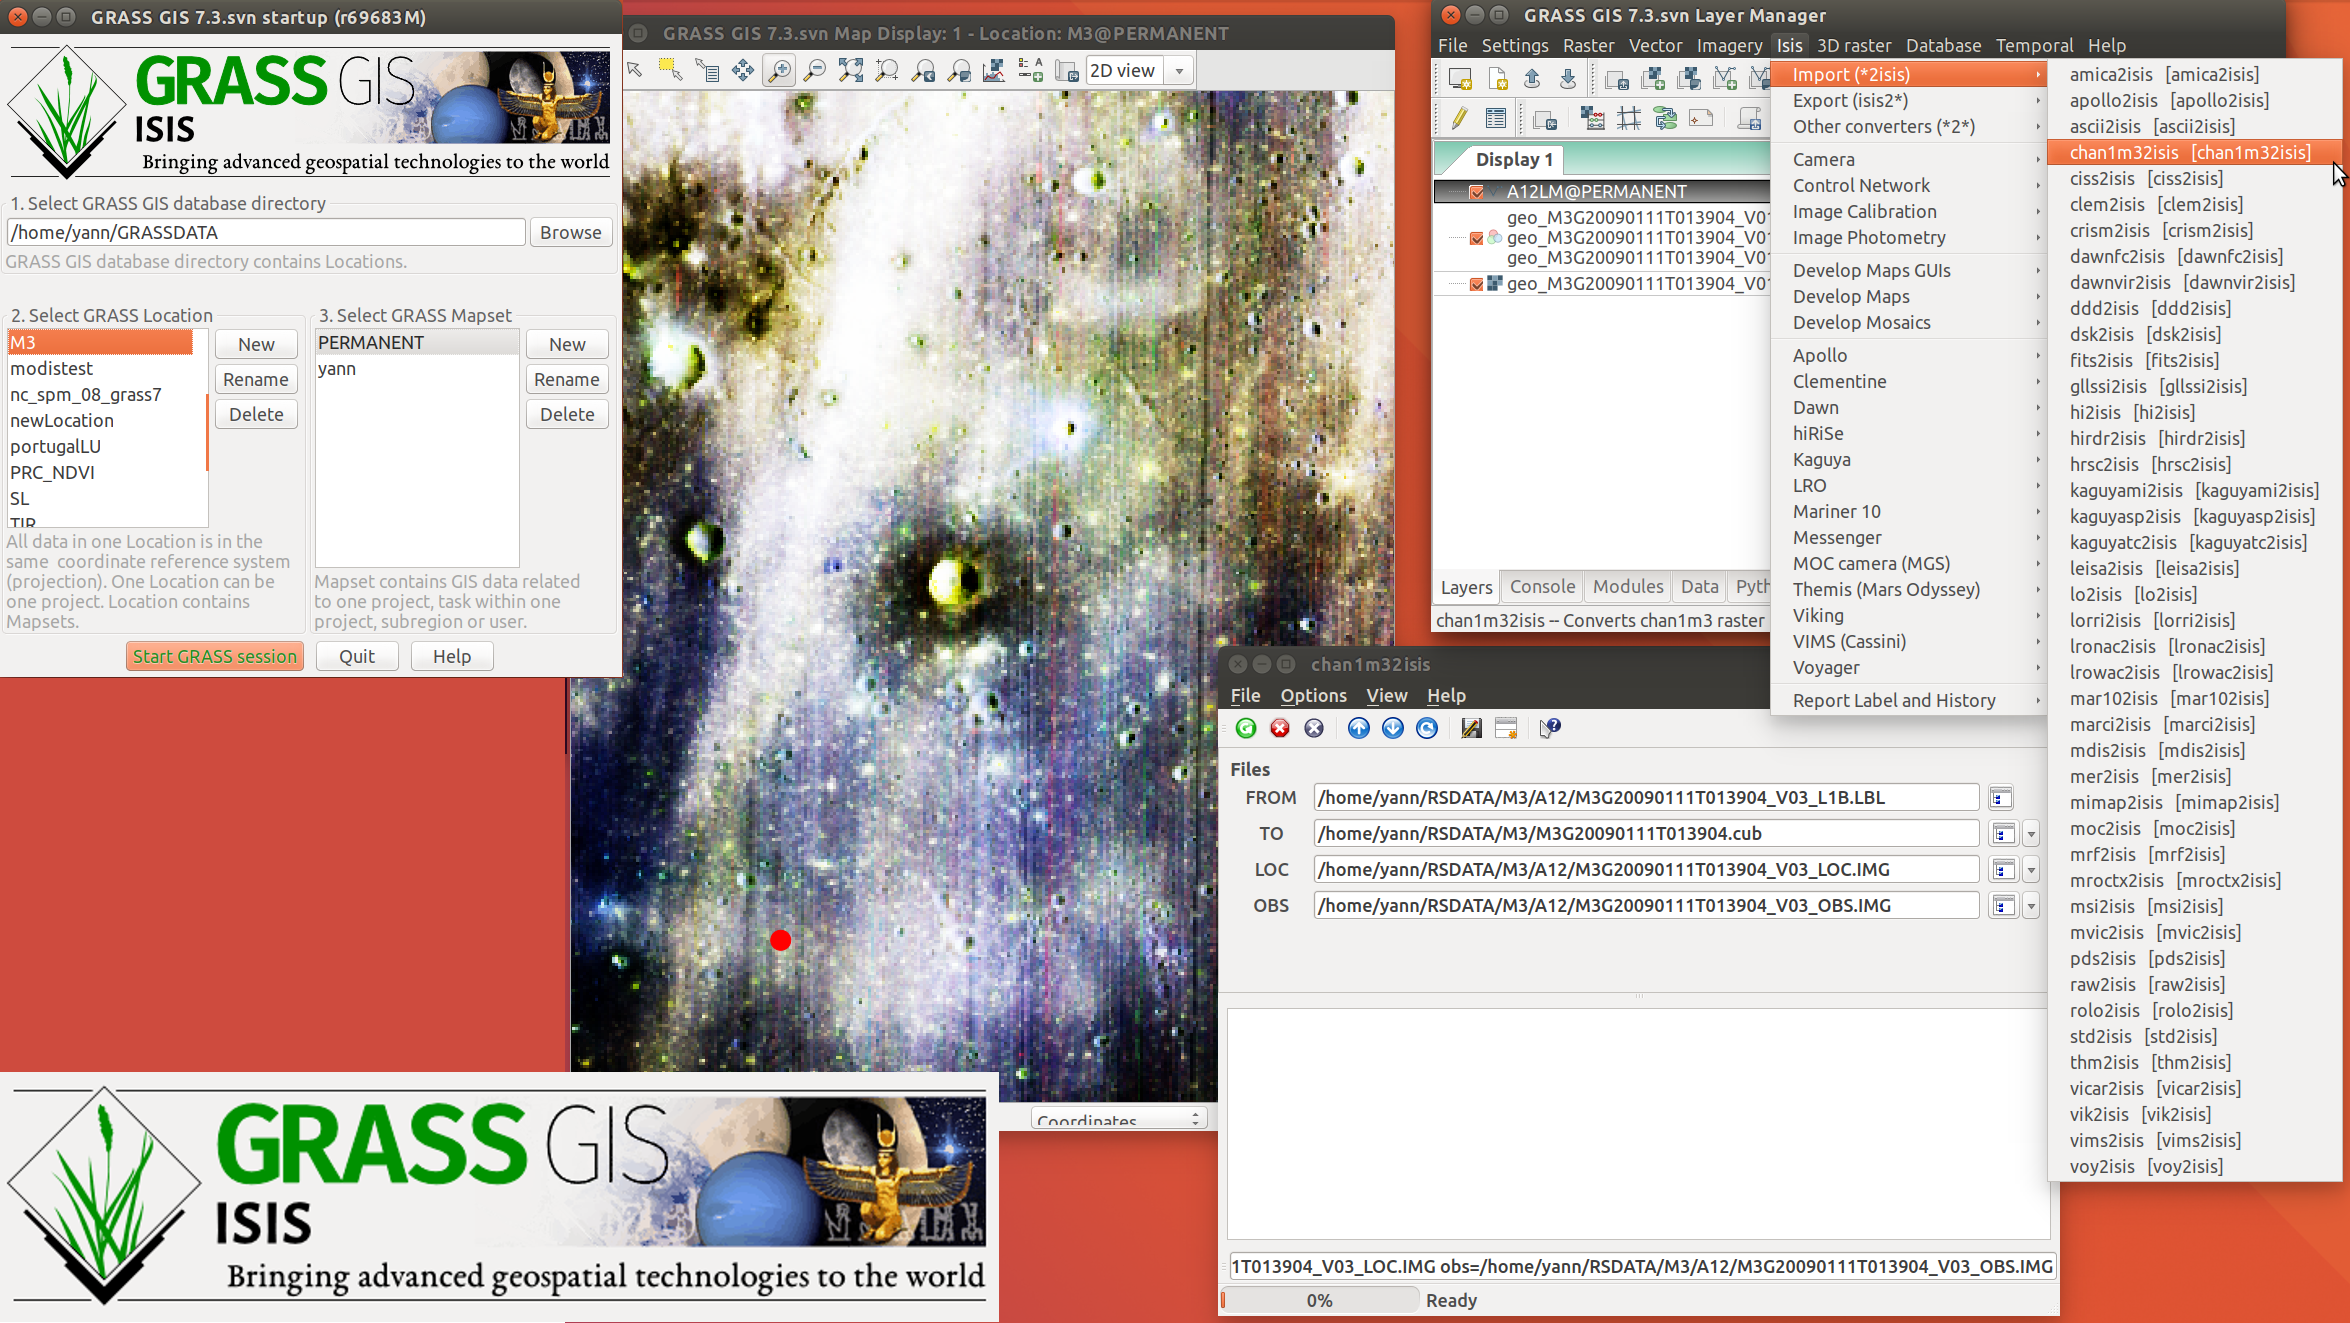
\includegraphics[width=12cm]{images/ISISwithGRASS}
 % \end{center}
\end{frame}}
%%%%%%%%%%%%%%%%%%%%%%%%%%%%%%%%%%%%%%%%%%%%%%%%%%%%%%%%%%%%%%%%%%%%
\begin{frame}[fragile]{M$^3$ part1}
\subsection{Craters location map}
\begin{center}
  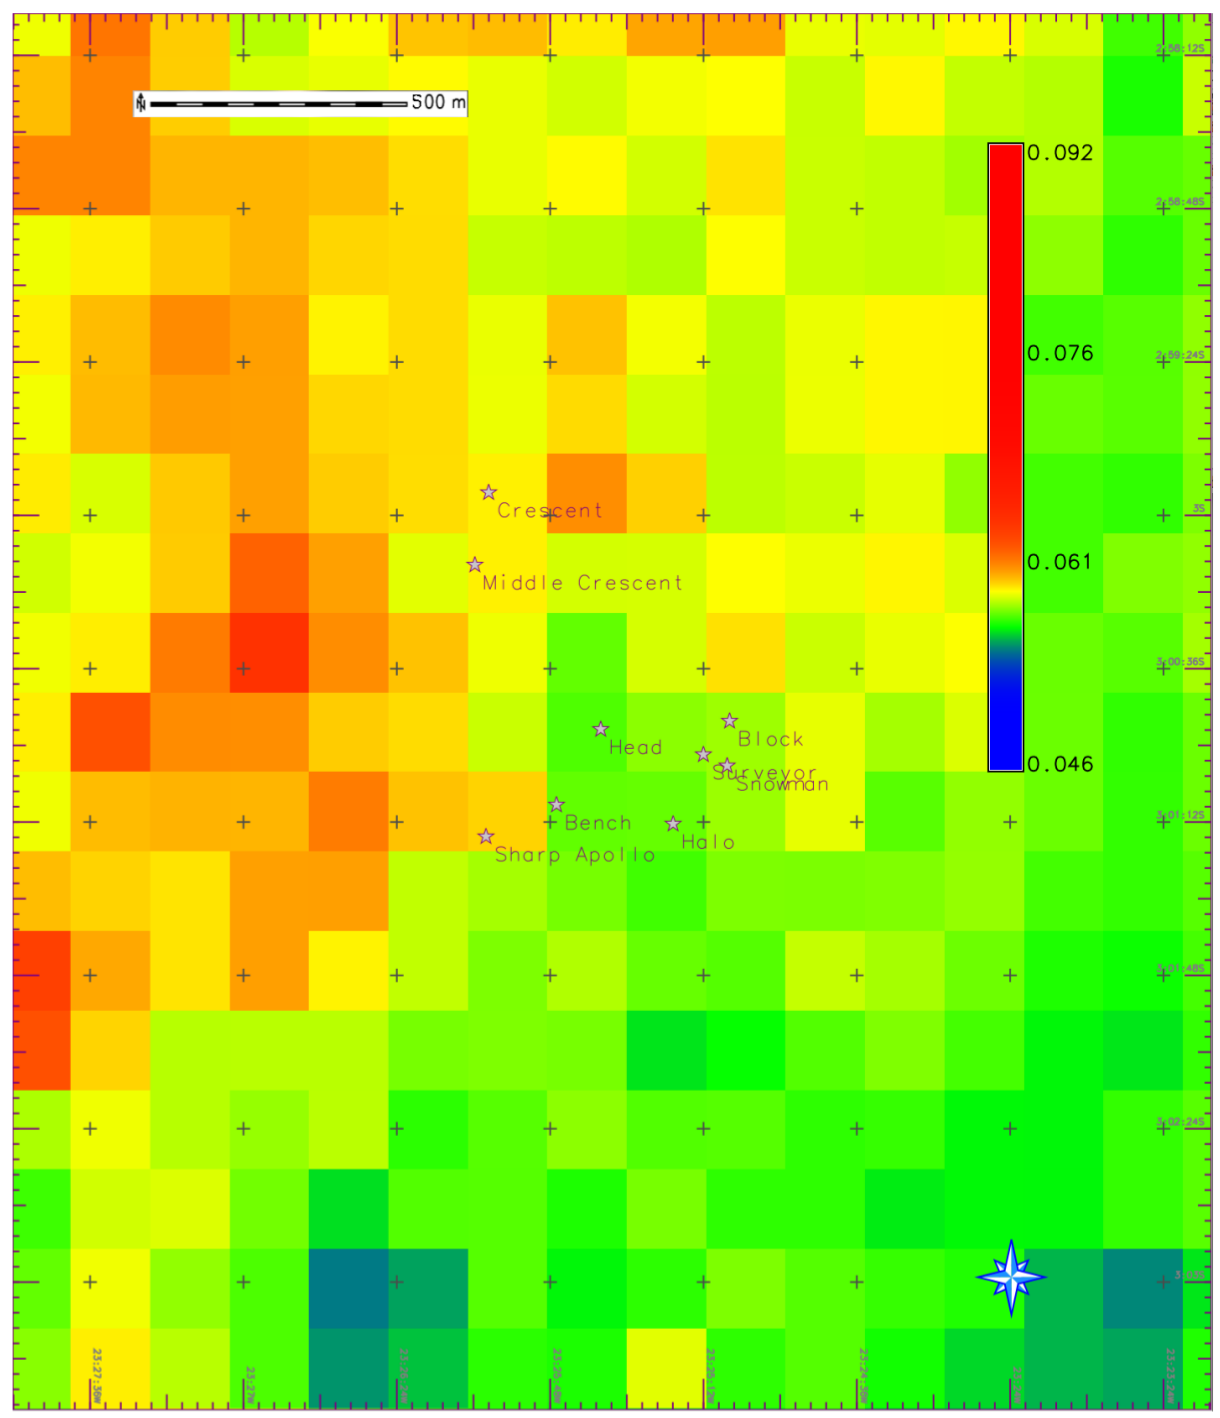
\includegraphics[width=6cm]{images/fig3}\\
  Crater location map (M$^3$ band 19, reflectance @ 950nm)
  \end{center}
\end{frame}
%%%%%%%%%%%%%%%%%%%%%%%%%%%%%%%%%%%%%%%%%%%%%%%%%%%%%%%%%%%%%%%%%%%%
\begin{frame}[fragile]{M$^3$ part2}
\subsection{Craters hyperspectral signal}
\begin{center}
  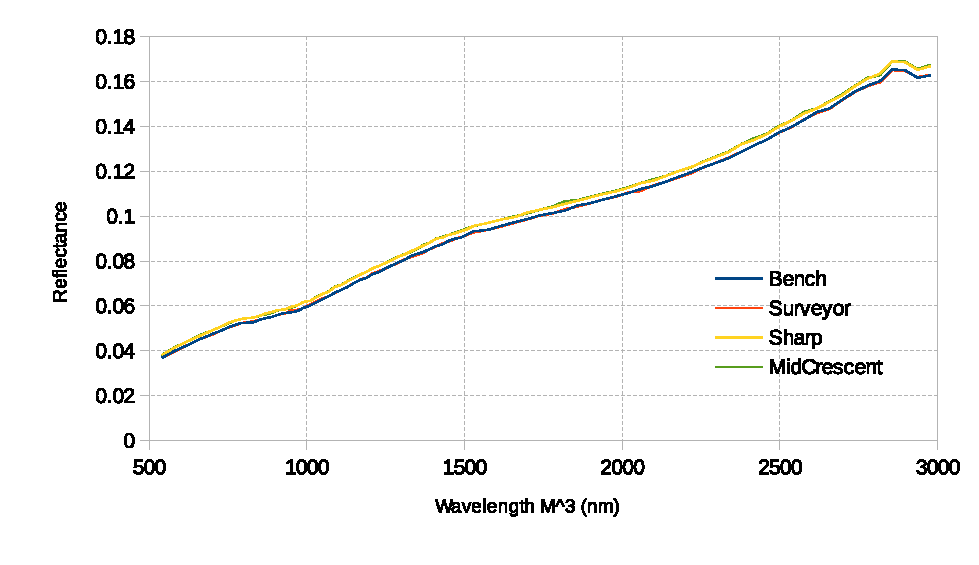
\includegraphics[width=12cm]{images/fig4}\\
  A12 Craters hyperspectral signal
  \end{center}
\end{frame}

%%%%%%%%%%%%%%%%%%%%%%%%%%%%%%%%%%%%%%%%%%%%%%%%%%%%%%%%%%%%%%%%%%%%
\begin{frame}[fragile]{M$^3$ part3}
\begin{center}
  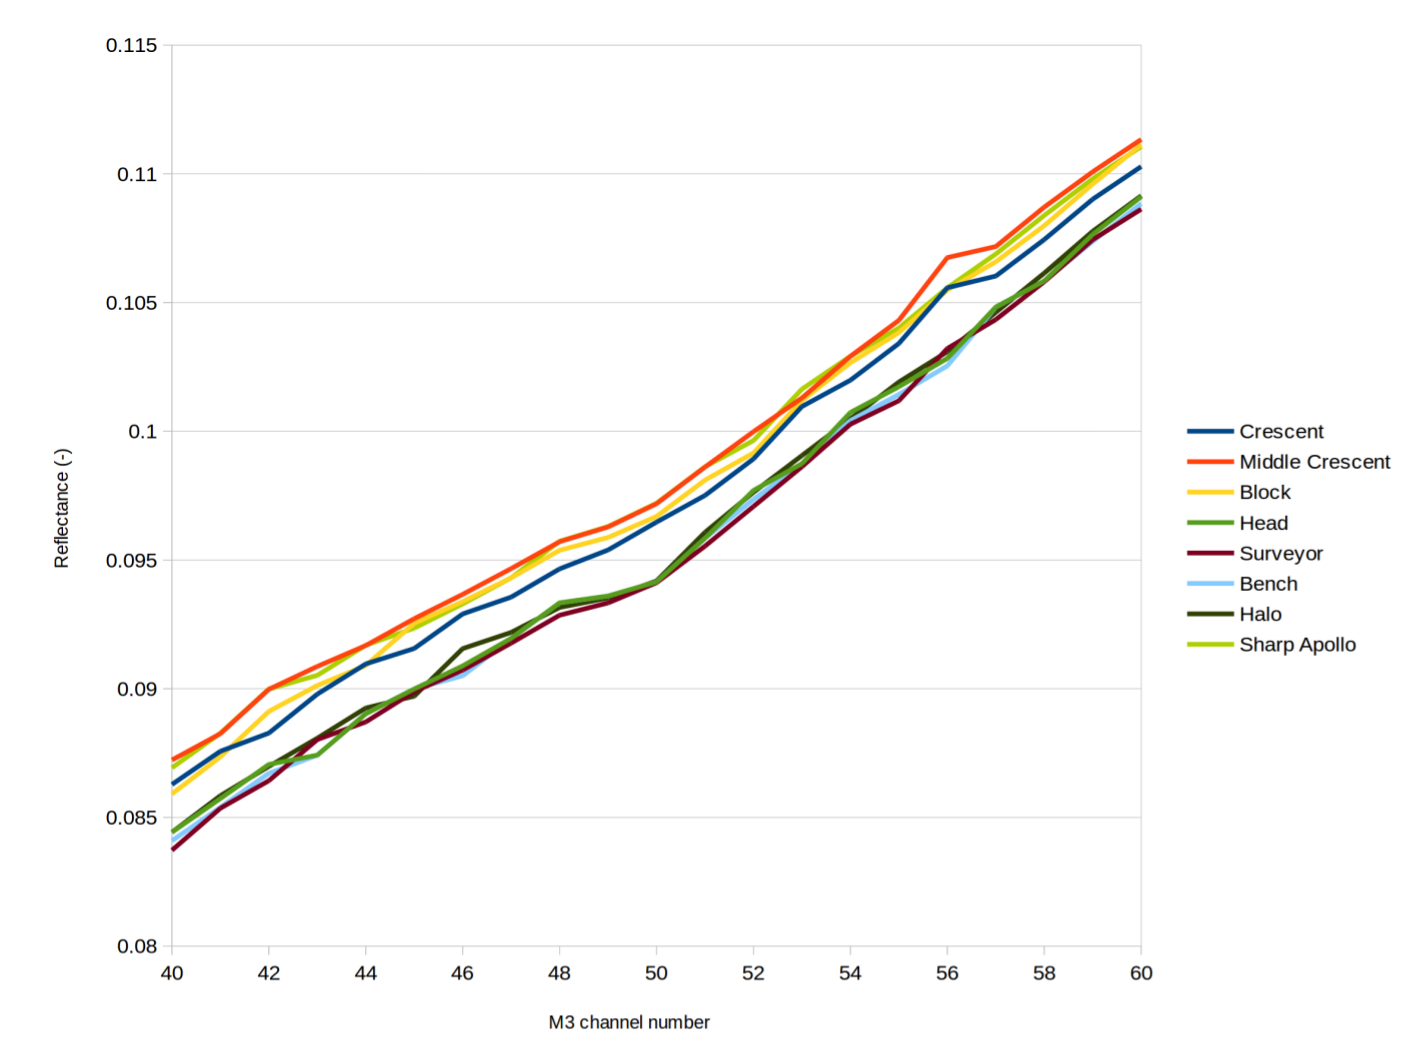
\includegraphics[width=9cm]{images/fig5}\\
  A12 Craters hyperspectral signal Zoom
  \end{center}
\end{frame}

\section{Methods and results}
%%%%%%%%%%%%%%%%%%%%%%%%%%%%%%%%%%%%%%%%%%%%%%%%%%%%%%%%%%%%%%%%%%%%
\begin{frame}[fragile]{Zhangetal}
\subsection{FeO Mapping}
\begin{block}{FeO equation}
\begin{itemize}
\item Derived from Clementine work and type of equation
\item Performs well regionally
\item Zhang and Bowles [2013]*
\item Made a GRASS GIS v7 Add-on: i.feotio2
\item FeO and TiO$_{2}$ equations for Clementine and Chan1-M$^3$
\end{itemize}
\end{block}
\begin{block}{}
\begin{equation}\label{zhang2013corrected}
 \theta_{Fe} [wt\%] = -arctan \left[ \frac {\frac {R_{950}} {R_{750}} - 1.26} {R_{750} - 0.01} \right]
\end{equation}
\end{block}
[*]{\small Zhang, W. Bowles, N.E. \textit{Mapping lunar TiO$_{2}$ and FeO with Chandrayaan-1 M$^3$ data}. In
Lunar and Planetary Institute Science Conference Abstracts, volume 44, page 1212,
2013.}
\end{frame}

%%%%%%%%%%%%%%%%%%%%%%%%%%%%%%%%%%%%%%%%%%%%%%%%%%%%%%%%%%%%%%%%%%%%
\begin{frame}[fragile]{Zhangetal}
\subsection{Zhang et al. corrected}
\begin{center}
  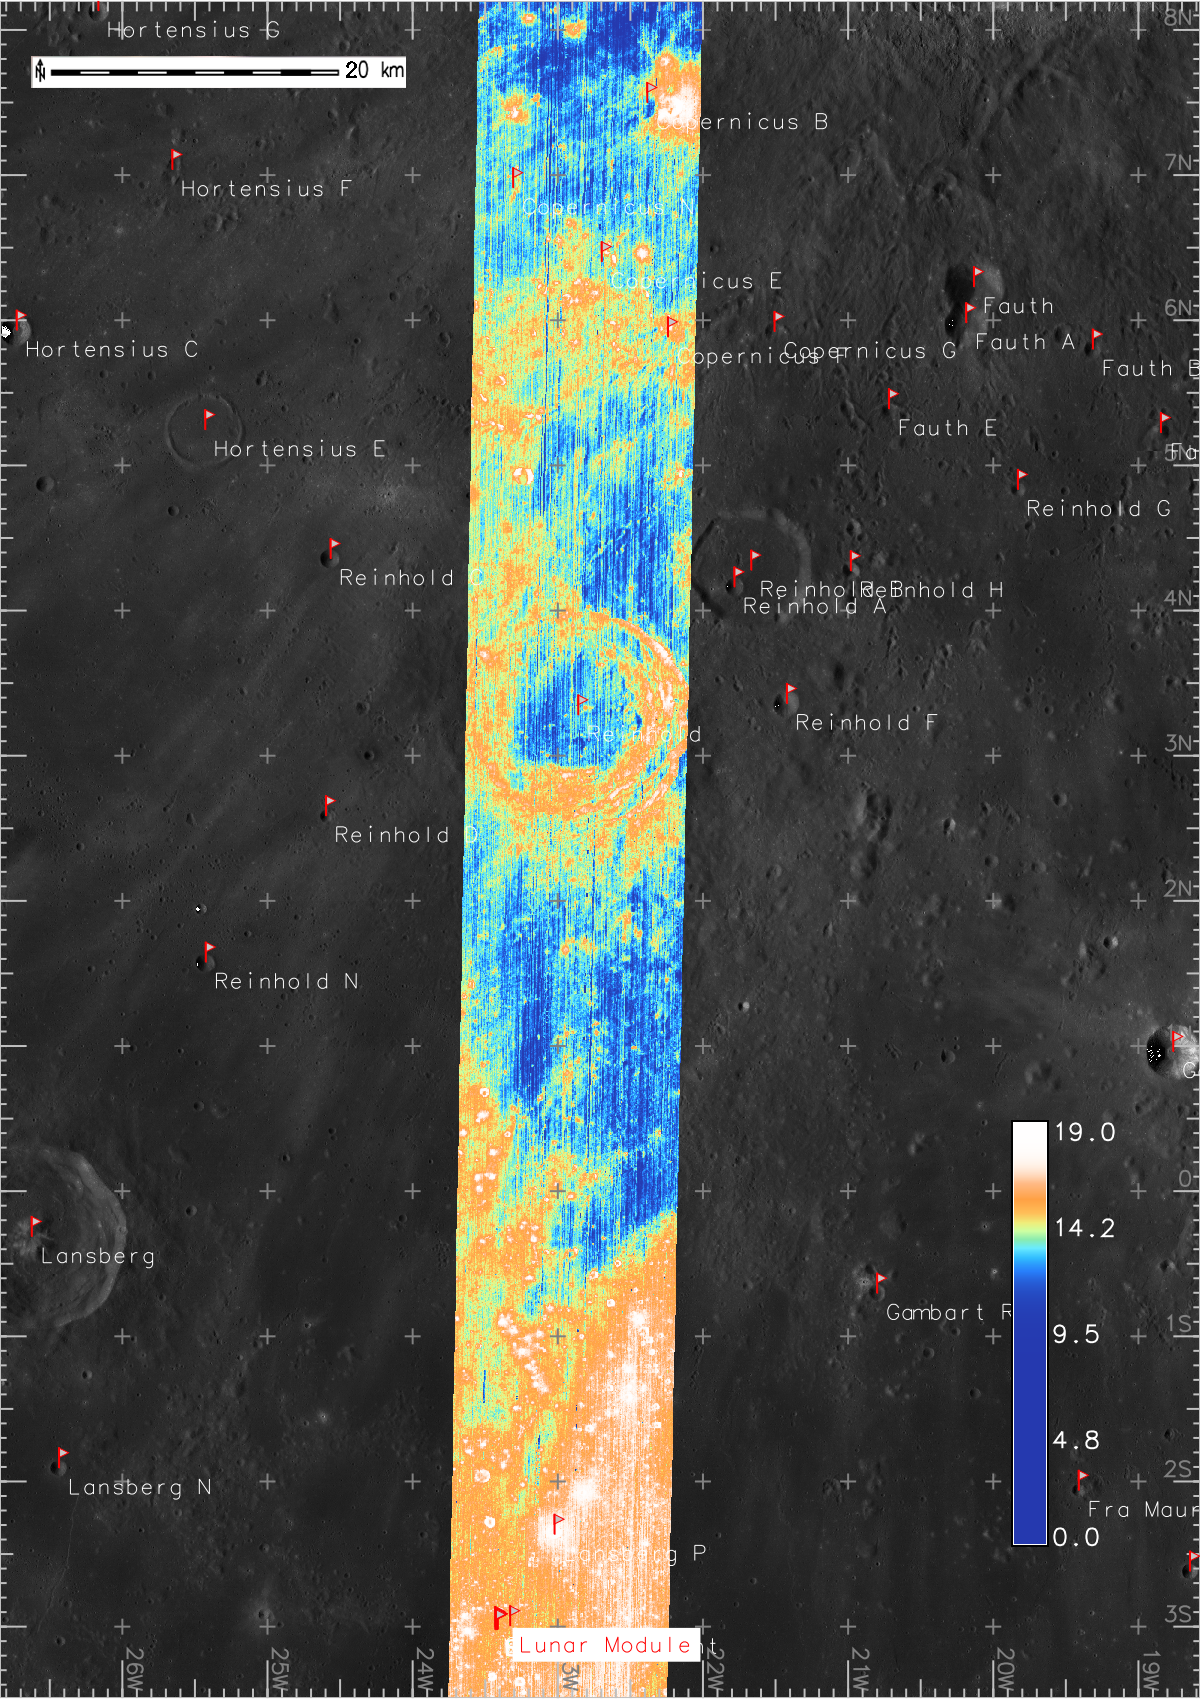
\includegraphics[width=5cm]{images/fig7}\\
  Zhang et al [2013] FeO[wt\%]
  \end{center}
\end{frame}

%%%%%%%%%%%%%%%%%%%%%%%%%%%%%%%%%%%%%%%%%%%%%%%%%%%%%%%%%%%%%%%%%%%%
\begin{frame}[fragile]{Segmentation}
\subsection{Object-based classification}
\begin{block}{Object-based classification}
\begin{itemize}
\item Classification based on both spectral and region growth statistics
\item Removed M$^3$ band 1 \& 2 as empty
\item Configured to simplify large regions instead of small units
\item Trying to exploit the reflectance gap in craters signal
\item Momsen and Metz [2012]* 
\item GRASS GIS: i.segment
\end{itemize}
\end{block}
[*]{\small Momsen, E., Metz, M. \textit{Object-oriented classification in GRASS GIS}, GSoC, 2012.}
\end{frame}


%%%%%%%%%%%%%%%%%%%%%%%%%%%%%%%%%%%%%%%%%%%%%%%%%%%%%%%%%%%%%%%%%%%%
\begin{frame}[fragile]{M$^3$ part3}
\begin{center}
  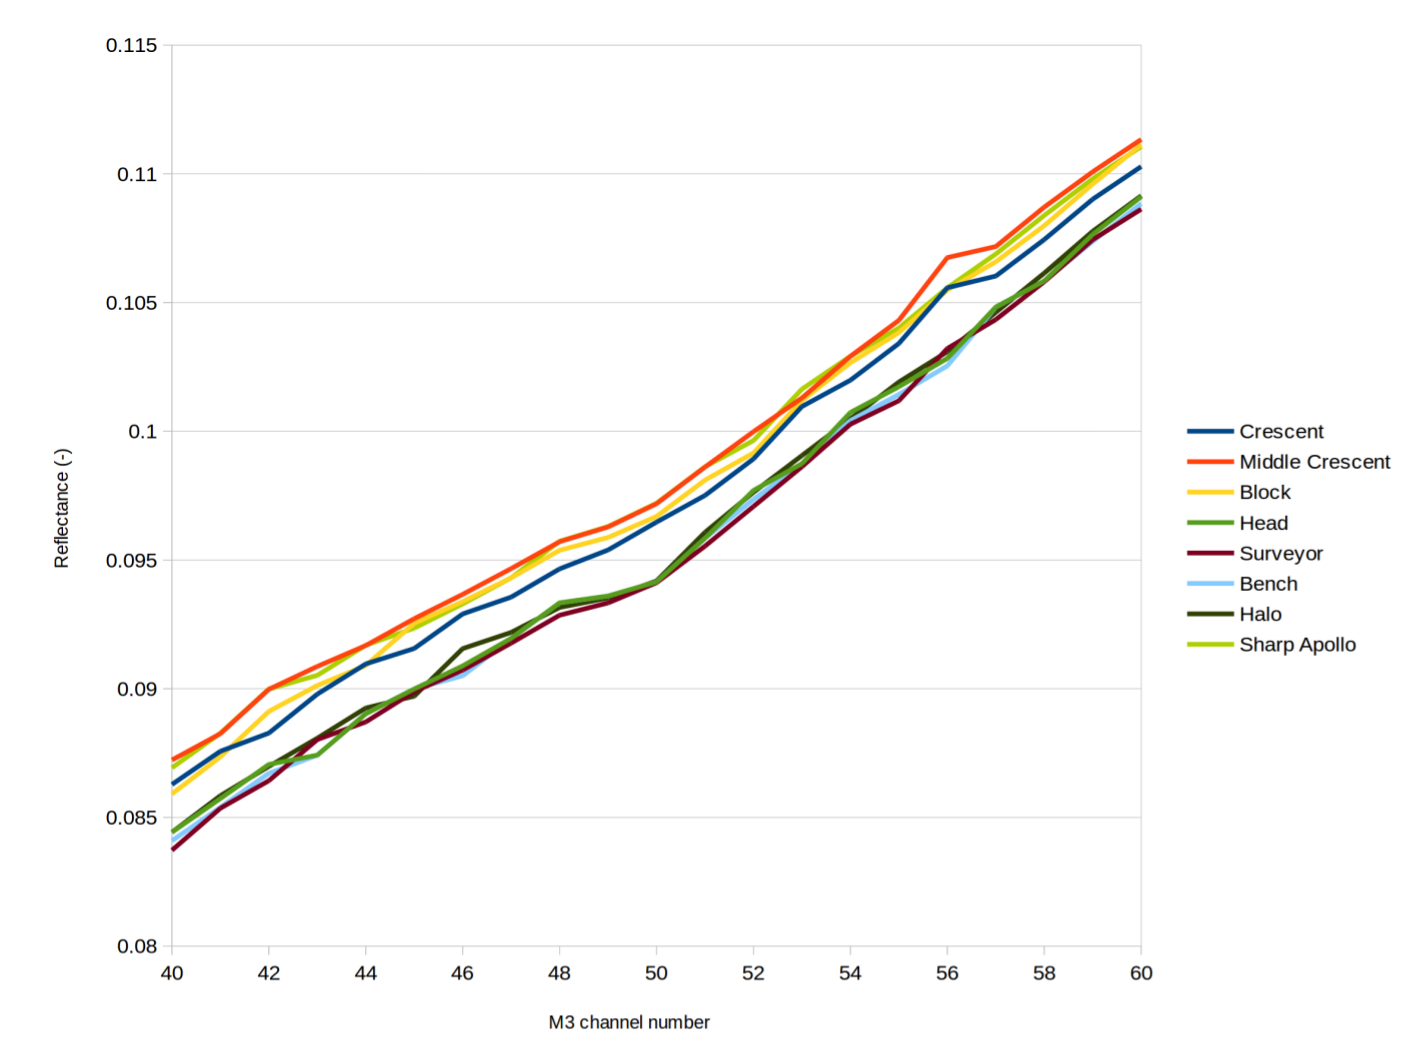
\includegraphics[width=9cm]{images/fig5}\\
  A12 Craters hyperspectral signal gap
  \end{center}
\end{frame}

%%%%%%%%%%%%%%%%%%%%%%%%%%%%%%%%%%%%%%%%%%%%%%%%%%%%%%%%%%%%%%%%%%%%
\begin{frame}[fragile]{i.segment}
\subsection{Relative Age Mapping}
\begin{center}
  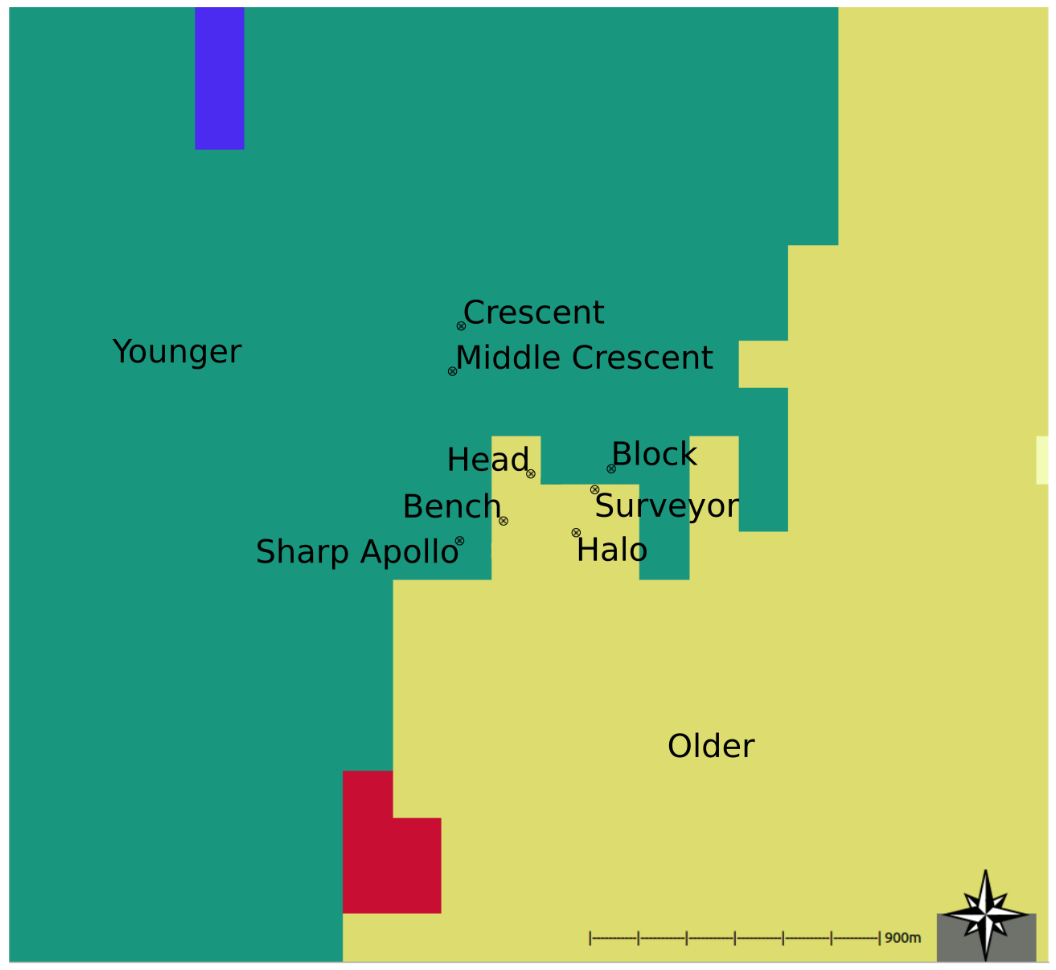
\includegraphics[width=7.5cm]{images/fig6}\\
  Object-based classification
  \end{center}
\end{frame}

%%%%%%%%%%%%%%%%%%%%%%%%%%%%%%%%%%%%%%%%%%%%%%%%%%%%%%%%%%%%%%%%%%%%
\begin{frame}[fragile]{Manual seek and compare}
\subsection{Manual seek and compare}
\begin{block}{Manual seek and compare}
\begin{itemize}
\item Compare each Relab signal from Apollo 12 to M$^3$
\item Removed M$^3$ band 1 \& 2 as empty
\item Closest found are half glass half rock (12063,79NT)
\item M$^3$ signal too linear
\end{itemize}
\end{block}
\end{frame}

%%%%%%%%%%%%%%%%%%%%%%%%%%%%%%%%%%%%%%%%%%%%%%%%%%%%%%%%%%%%%%%%%%%%%
%\begin{frame}[fragile]{Classical hyperspectral mapping}
%\subsection{Hyperspectral mapping}
%\begin{block}{Classical hyperspectral mapping}
%\begin{itemize}
%\item Classification based on spectral statistics
%\item Removed M$^3$ band 1 \& 2 as empty
%\item Could separate end-members regionally
%\item Trying to exploit the Relab signatures (and others)
%\item M$^3$ signal too linear
%\end{itemize}
%\end{block}
%\end{frame}
%
%%%%%%%%%%%%%%%%%%%%%%%%%%%%%%%%%%%%%%%%%%%%%%%%%%%%%%%%%%%%%%%%%%%%%
%\begin{frame}[fragile]{Spectral angle mapping/unmixing}
%\subsection{Spectral angle mapping}
%\begin{block}{Spectral angle mapping/unmixing}
%\begin{itemize}
%\item Classification based on spectral angle statistics
%\item Removed M$^3$ band 1 \& 2 as empty
%\item Trying to exploit the Relab signatures
%\item Relab db to colinear, did not finish simplifying it (involves some stats).
%\item Closest Relab signal is 89 degrees from M$^3$...
%\end{itemize}
%\end{block}
%\end{frame}
%
%


%%%%%%%%%%%%%%%%%%%%%%%%%%%%%%%%%%%%%%%%%%%%%%%%%%%%%%%%%%%%%%%%%%%%
\begin{frame}[fragile]{12063,79NT}
\subsection{Manual seek: 12063,79NT}
\begin{center}
  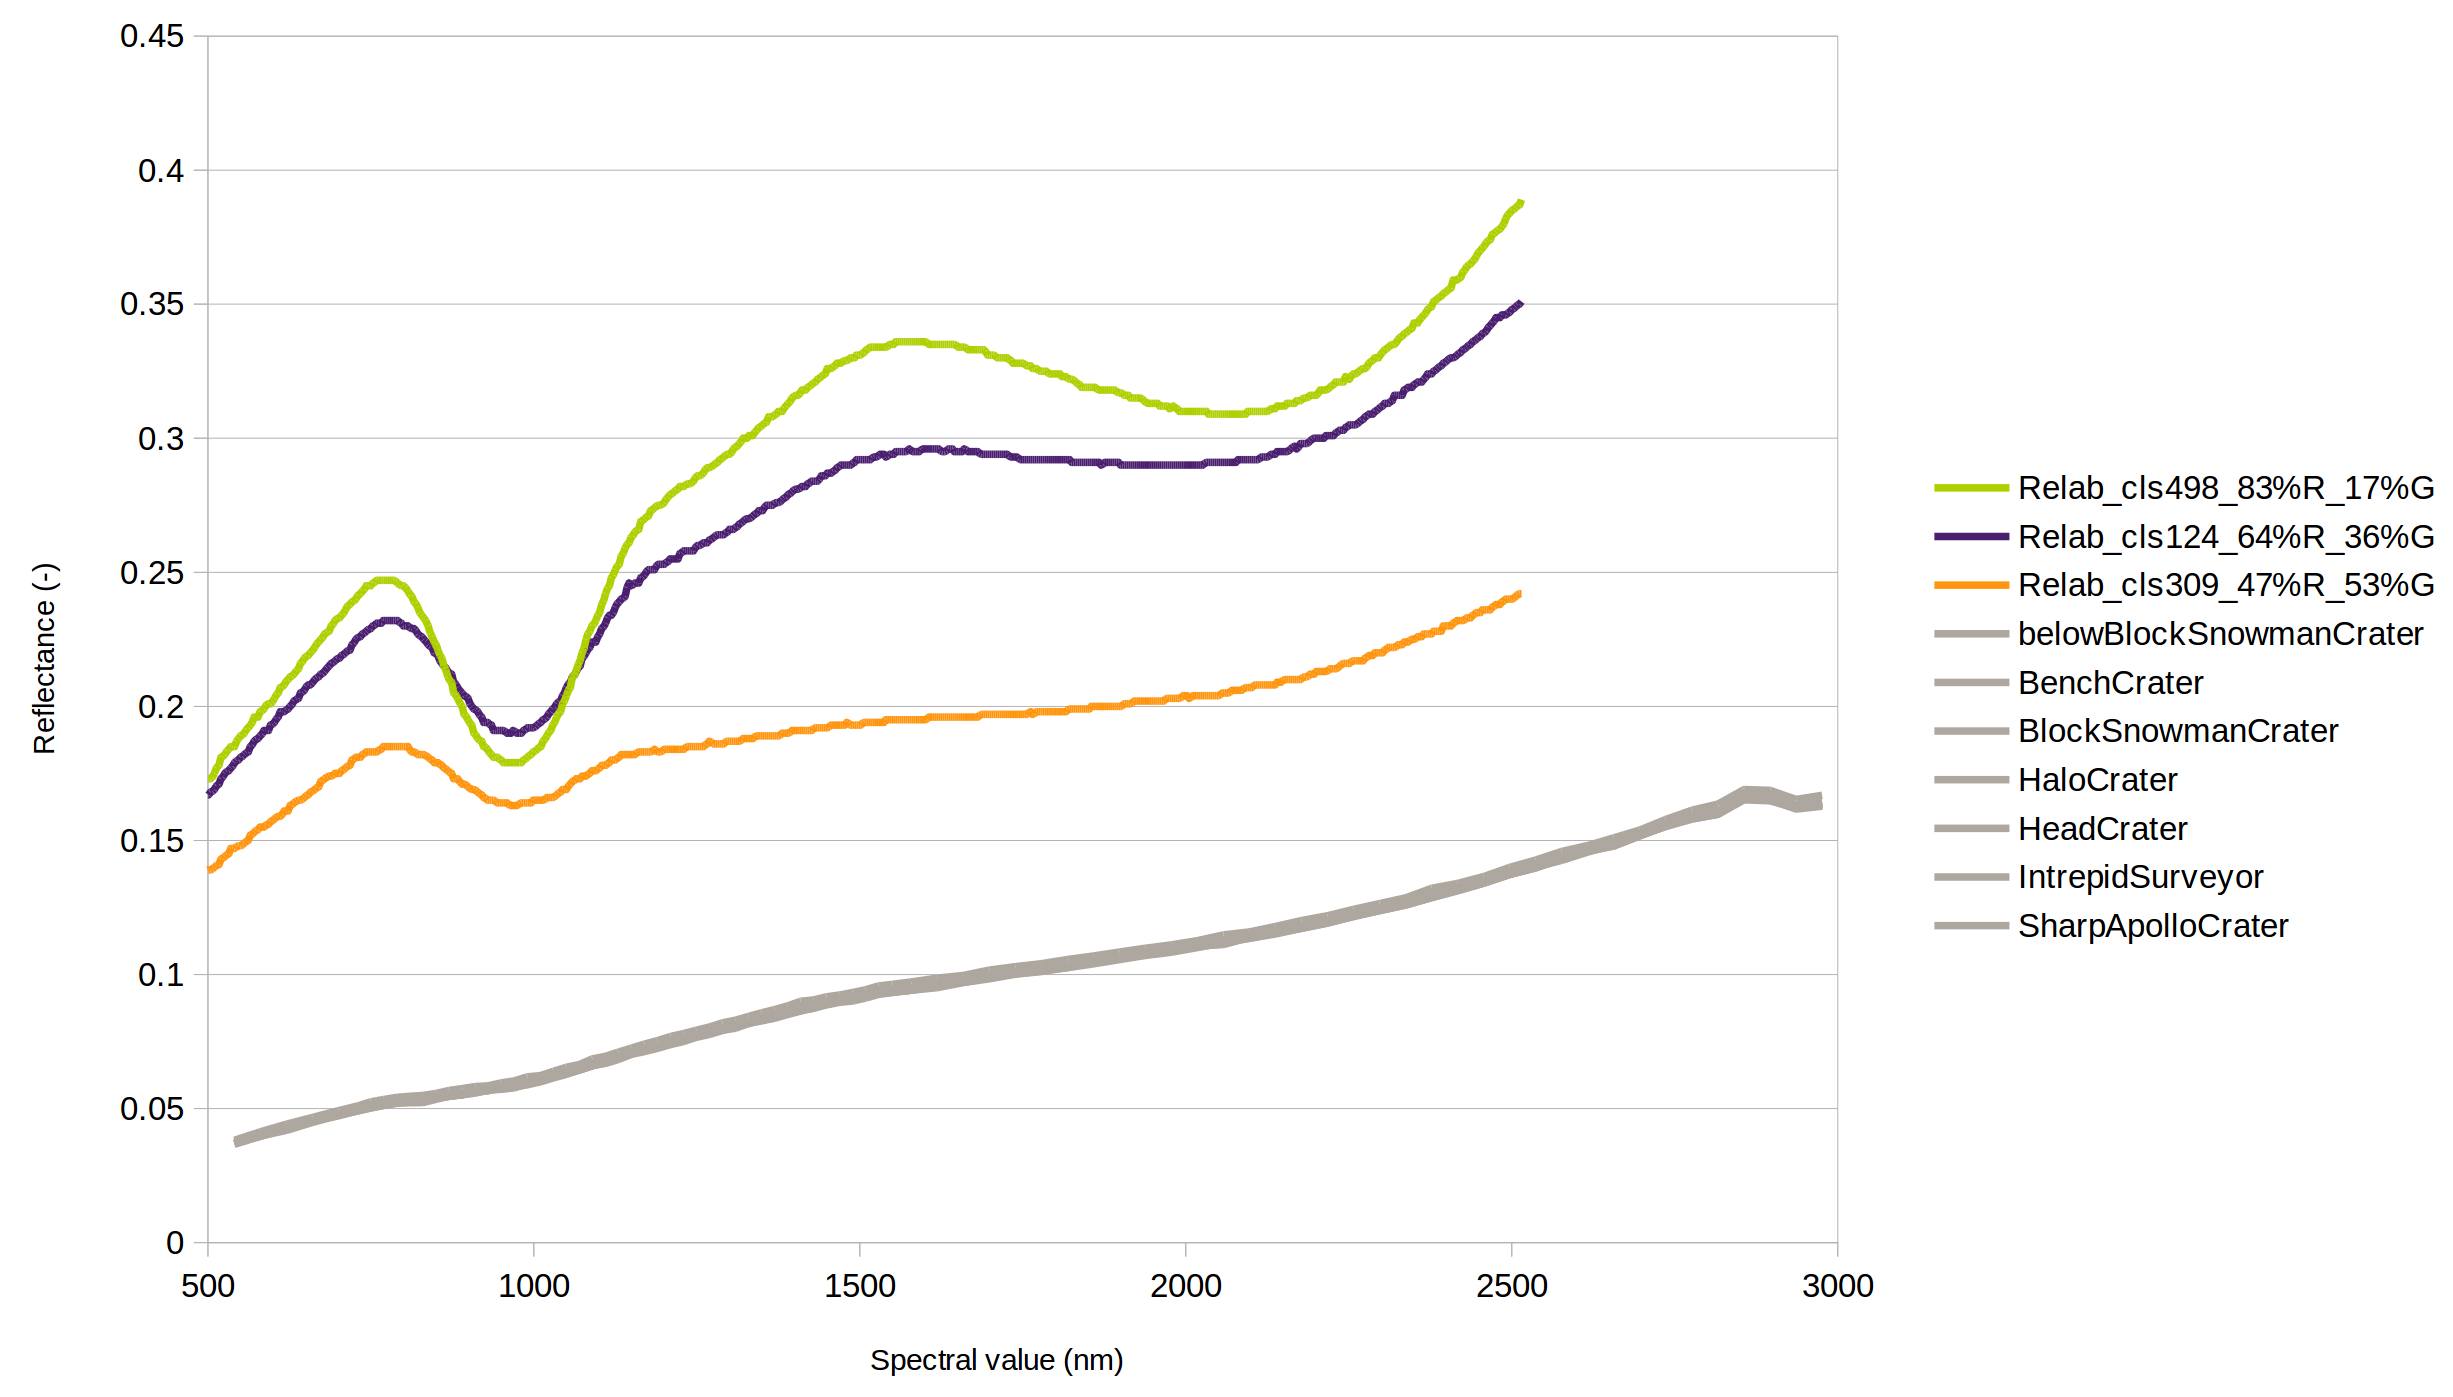
\includegraphics[width=12cm]{images/fig8}\\
  Manual seek: 12063,79NT (Relab cls309)
  \end{center}
\end{frame}

%%%%%%%%%%%%%%%%%%%%%%%%%%%%%%%%%%%%%%%%%%%%%%%%%%%%%%%%%%%%%%%%%%%%
\begin{frame}[fragile]{12063,79NT}
\begin{center}
  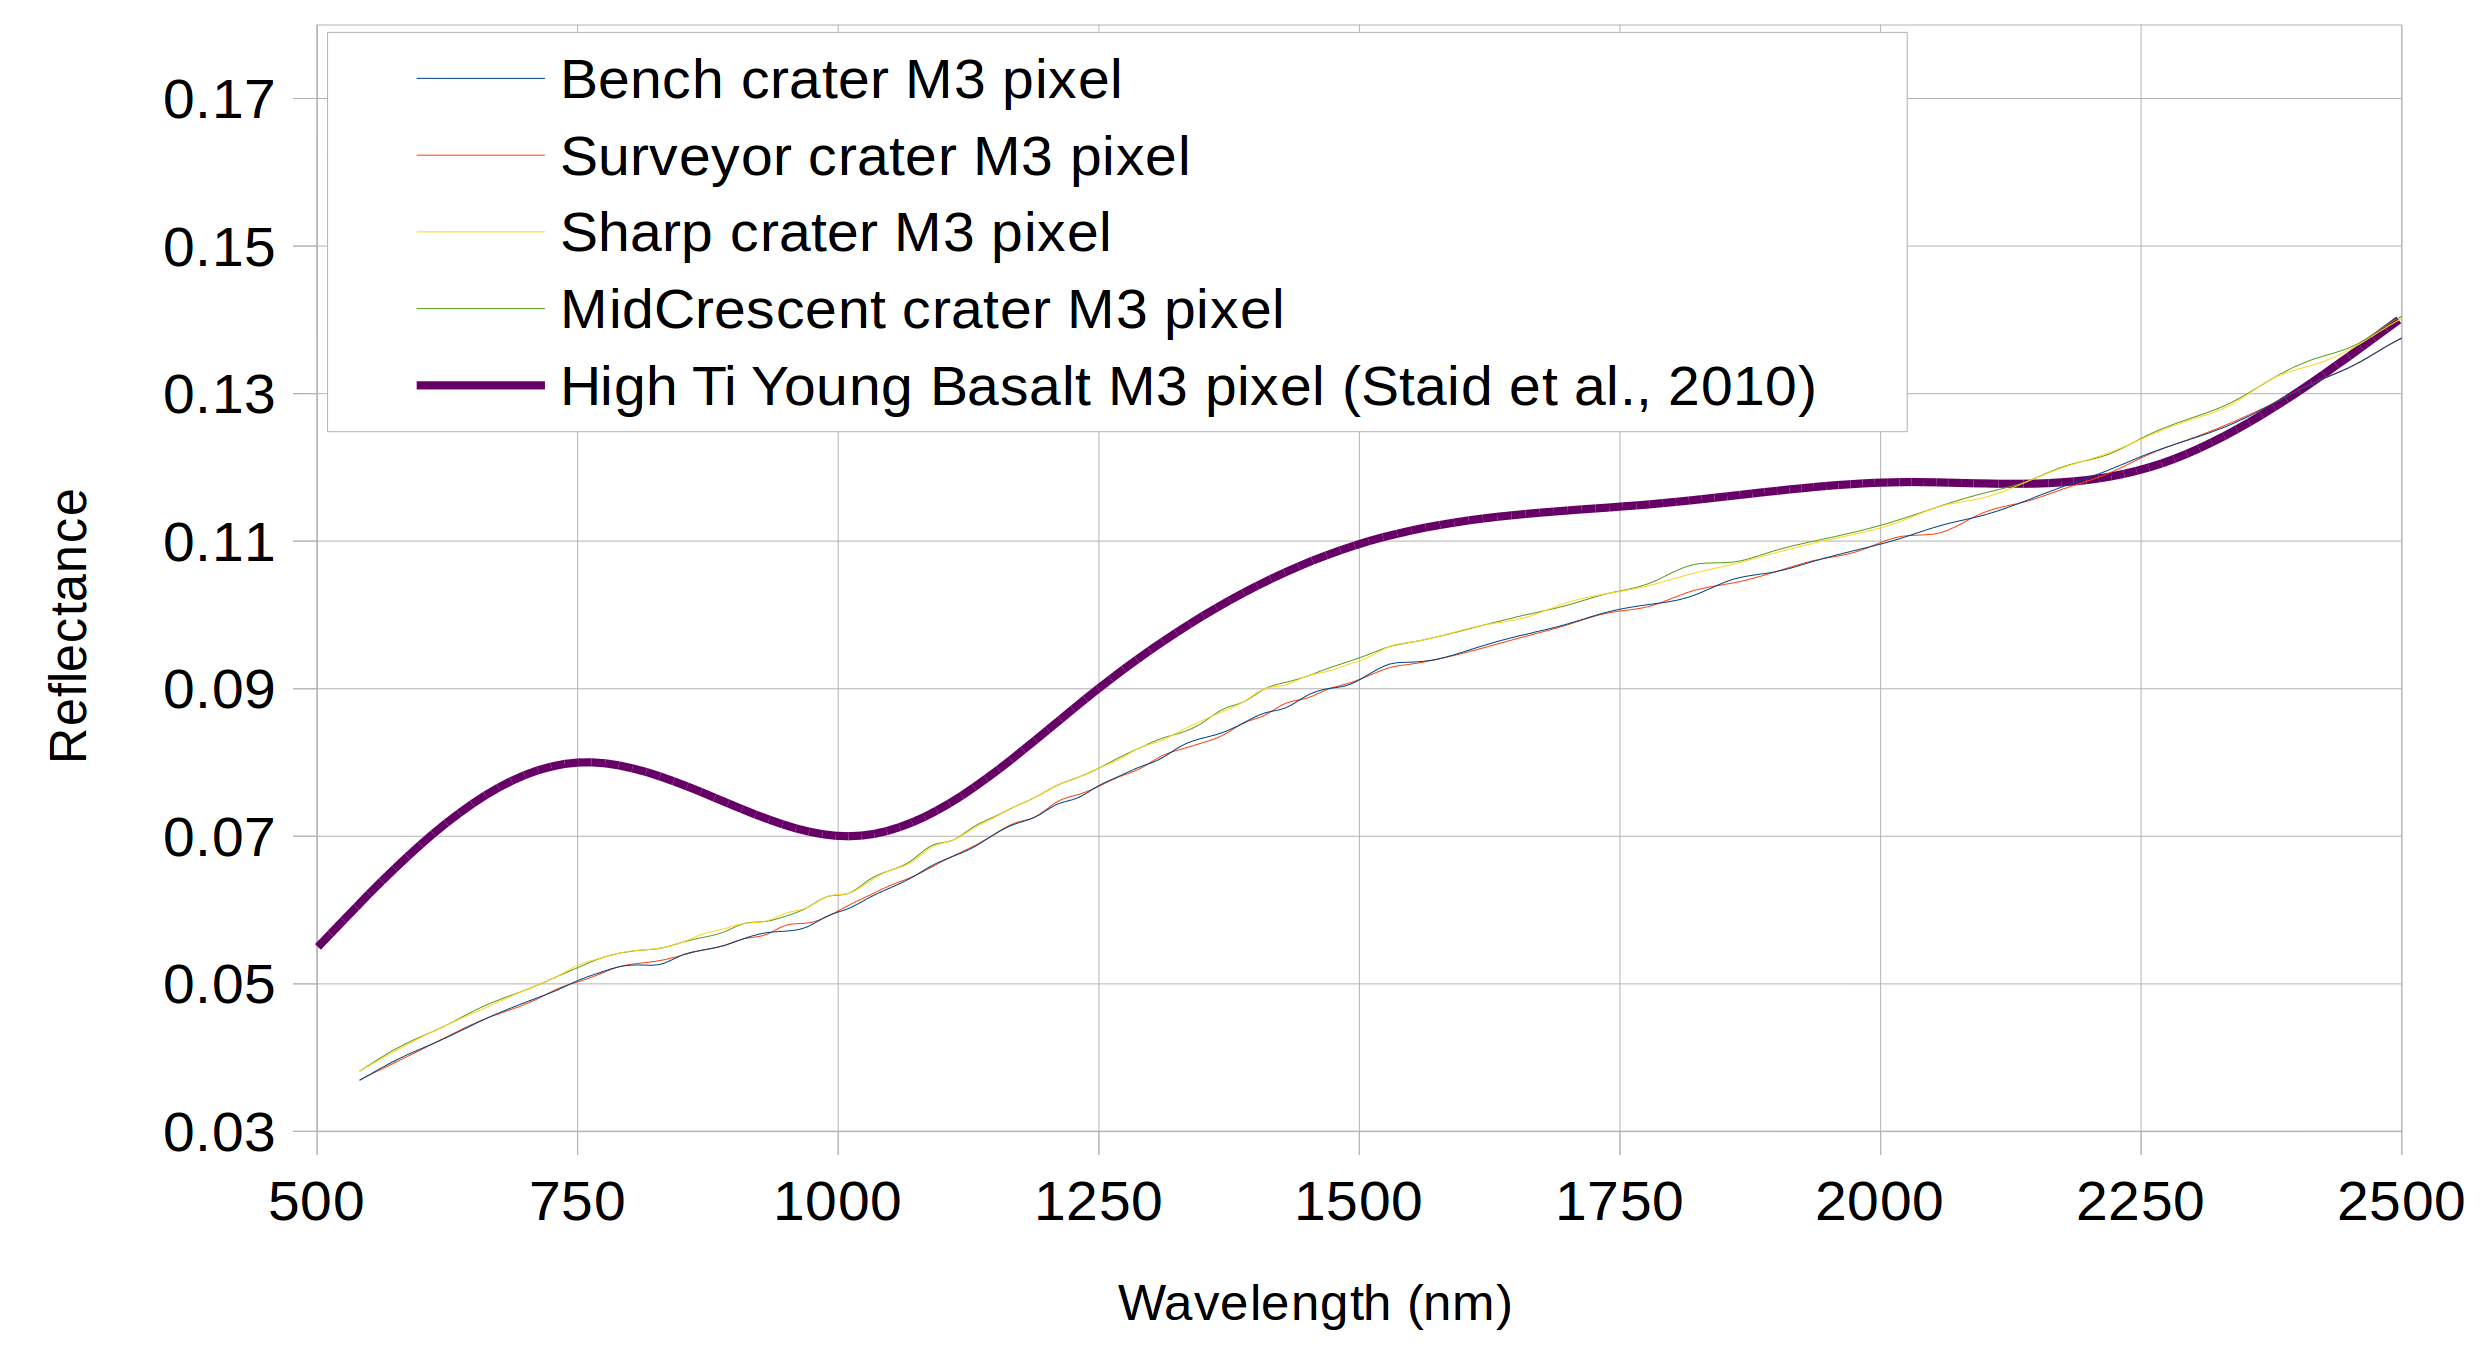
\includegraphics[width=12cm]{images/fig9}\\
  Manual seek: 12063,79NT compare Staid et al. [2011] Mare Basalt
  \end{center}
\end{frame}

%%%%%%%%%%%%%%%%%%%%%%%%%%%%%%%%%%%%%%%%%%%%%%%%%%%%%%%%%%%%%%%%%%%%
\begin{frame}[fragile]{12063,79NT}
\begin{center}
  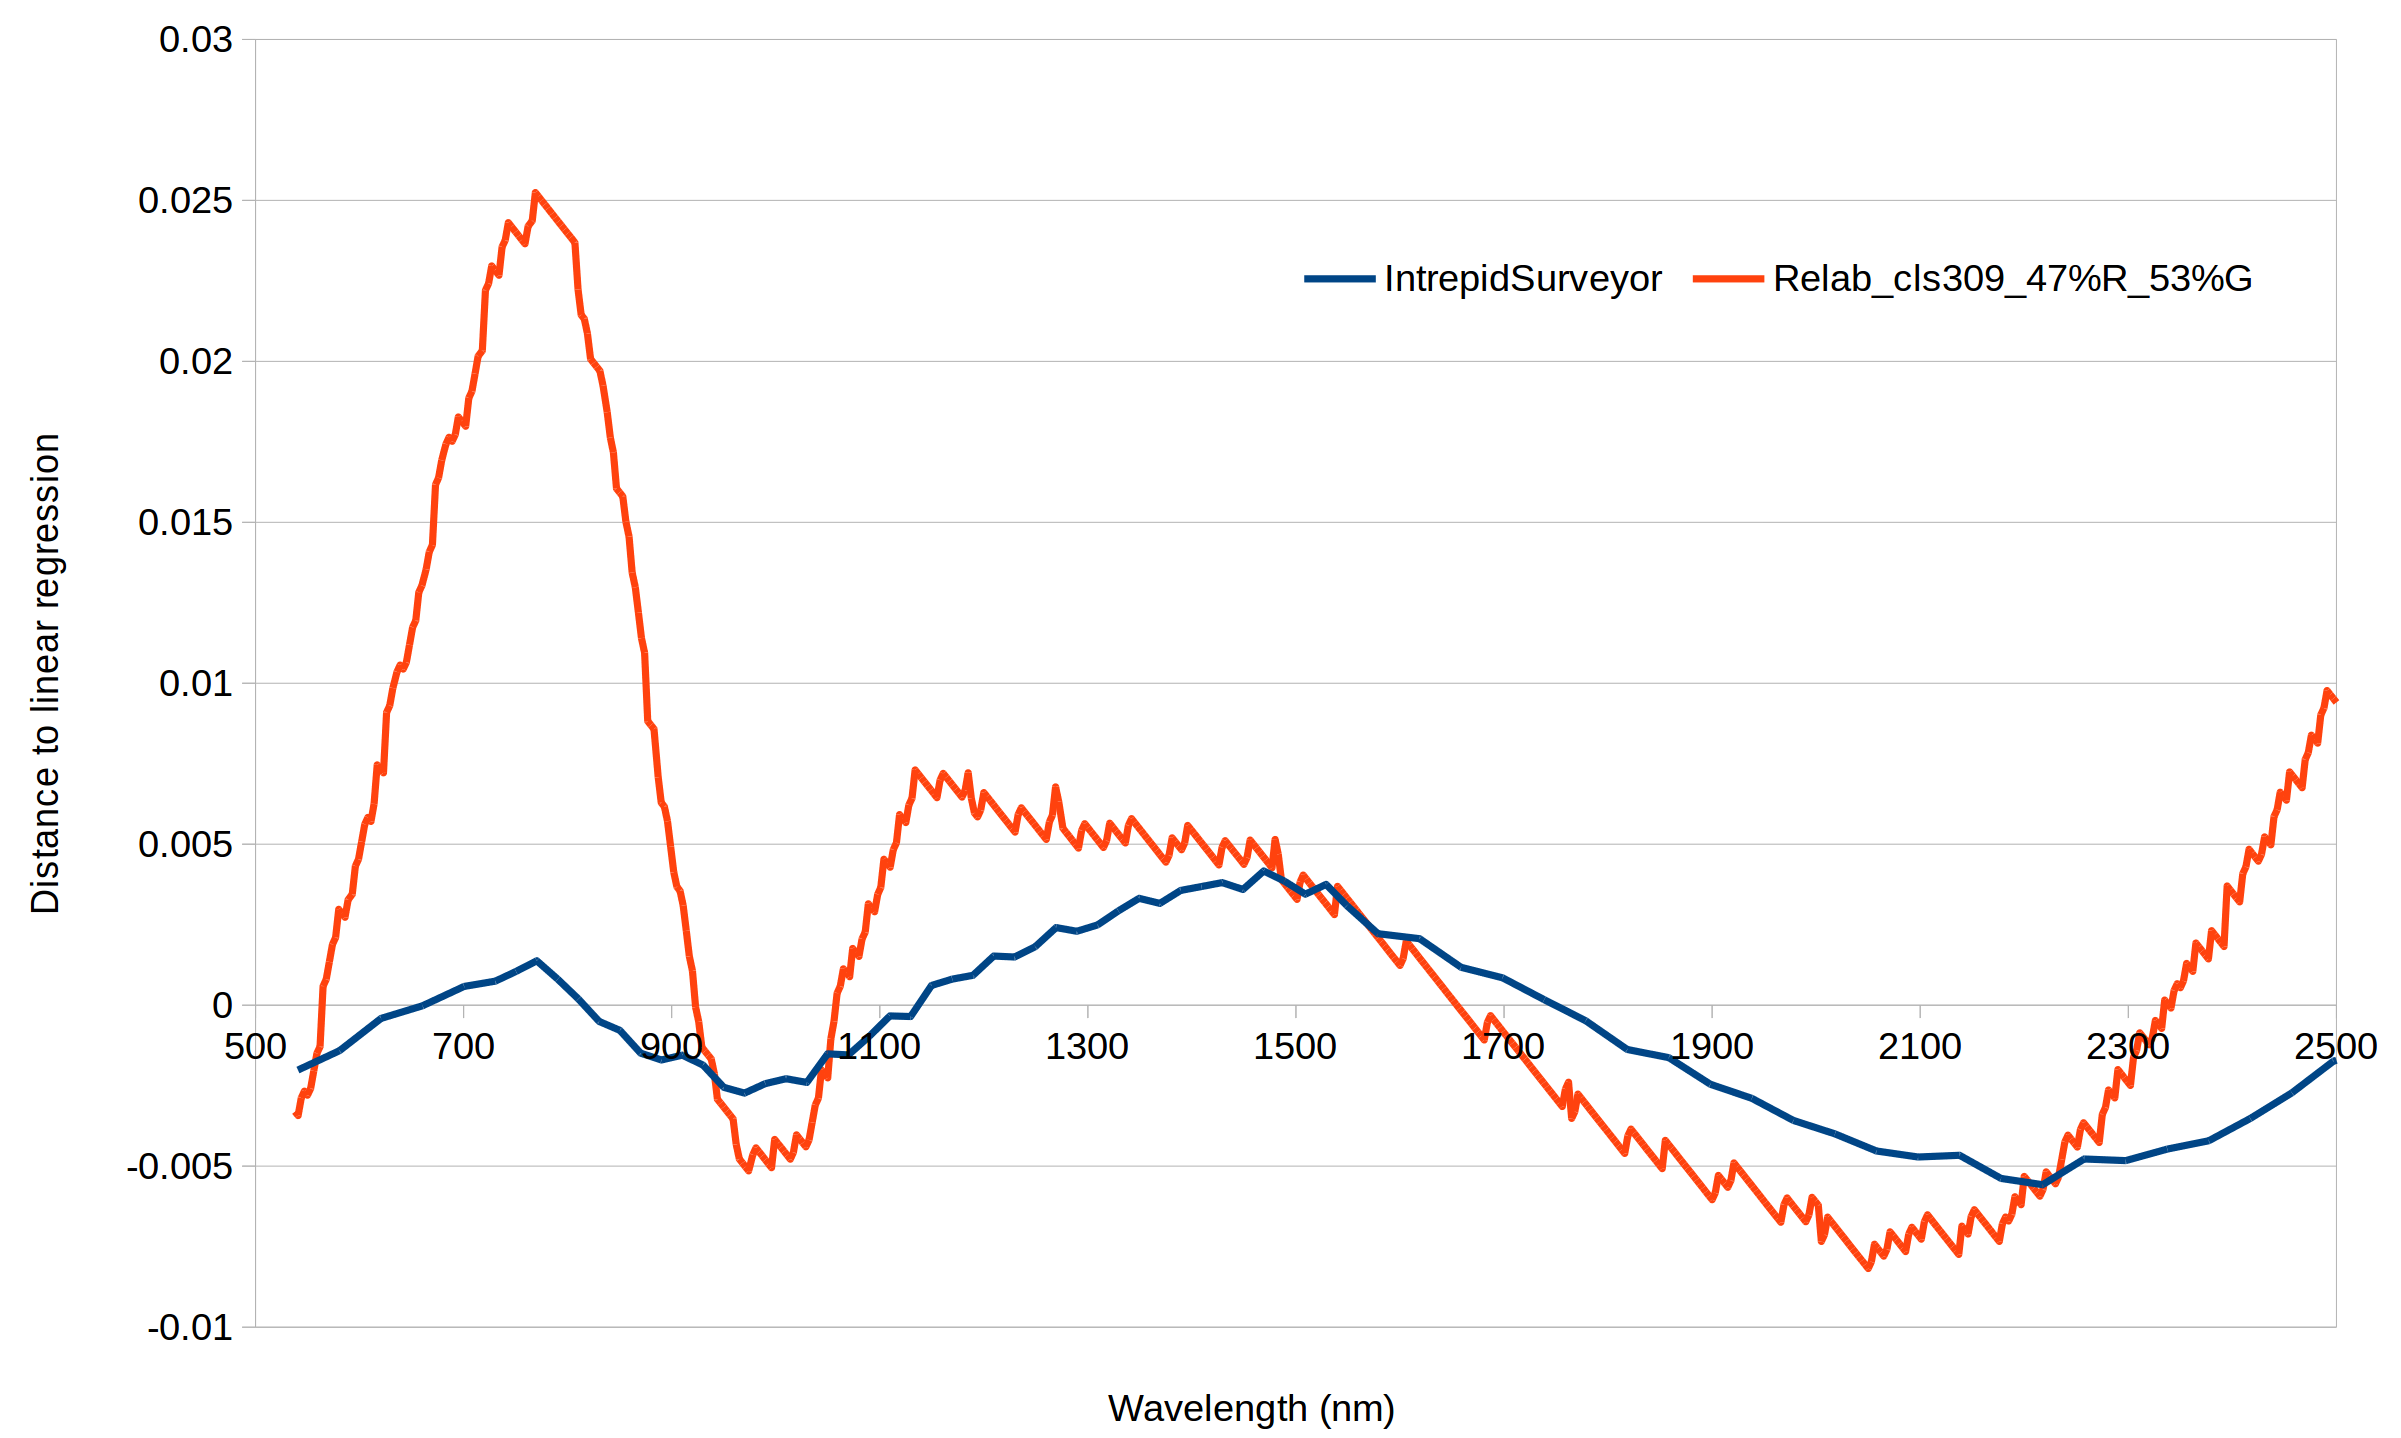
\includegraphics[width=11.5cm]{images/fig10}\\
  Manual seek: 12063,79NT compare Relab cls309 (detrended)
  \end{center}
\end{frame}

%%%%%%%%%%%%%%%%%%%%%%%%%%%%%%%%%%%%%%%%%%%%%%%%%%%%%%%%%%%%%%%%%%%%
\begin{frame}[fragile]{12063,79NT}
\begin{block}{Finding: CPX}
\begin{center}
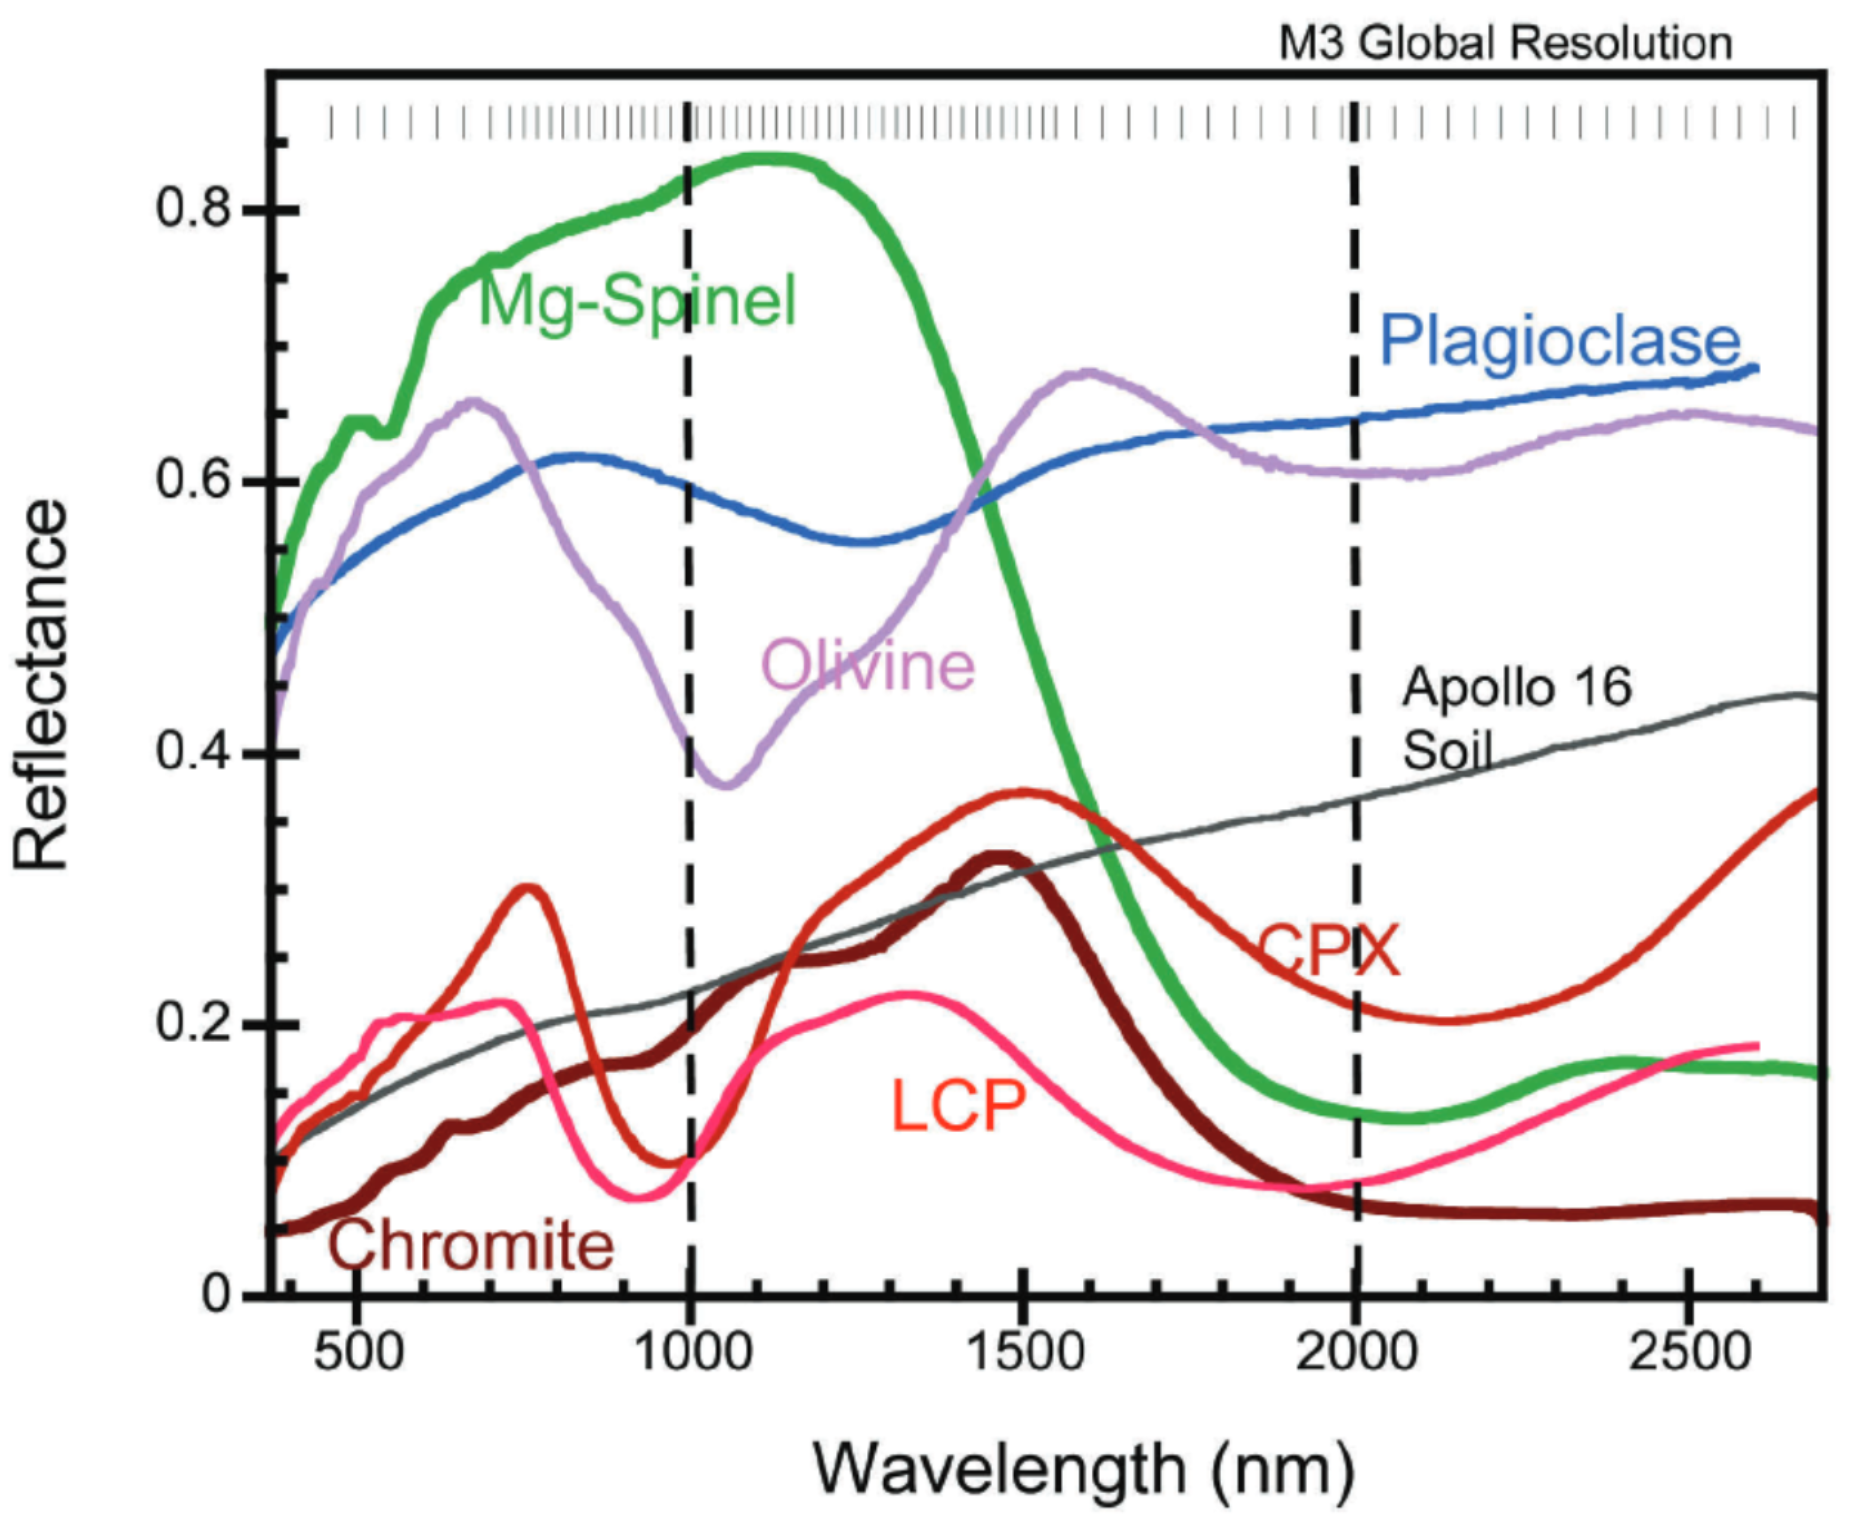
\includegraphics[width=7.5cm]{images/fig11}\\
Graph from Pieters et al. [2014]
\end{center}
\end{block}
\end{frame}

%%%%%%%%%%%%%%%%%%%%%%%%%%%%%%%%%%%%%%%%%%%%%%%%%%%%%%%%%%%%%%%%%%%%
\begin{frame}[fragile]{12063,79NT}
\begin{block}{Finding: CPX}
\begin{itemize}
\item \textbf{Pre-copernican}\\
Augite/pigeonite leaning towards Hedenbergite (CaFeSi$_2$O$_6$)
\item \textbf{Copernican}\\
Augite/pigeonite leaning towards Endiopside/Diopside (CaMgSi$_2$O$_6$)
\item Layer within 5000m in Copernicus crater (Pieters et al., 1985)*
\item Aging going out of the ray, increase FeO[wt\%]
\end{itemize}
\end{block}
[*]{\small Pieters, C.M., Adams, J.B., Mouginis-Mark, P.J., Zisk, S.H., Smith, M.O., Head, J.W., McCord, T.B. \textit{The nature of crater rays:
The copernicus example}. Journal of Geophysical Research: Solid Earth, 90(B14):12393–12413, 1985.}
\end{frame}

\section{Conclusions}
%%%%%%%%%%%%%%%%%%%%%%%%%%%%%%%%%%%%%%%%%%%%%%%%%%%%%%%%%%%%%%%%%%%%
\begin{frame}[fragile]{Conclusions}
\begin{block}{This study}
\begin{itemize}
\item Found some Copernican and pre-Copernican CPX
\item with FeO differences
\end{itemize}
\end{block}
\begin{block}{Future}
\begin{itemize}
\item 2018: Imaging IR Spectrometer on Chandrayaan-2 (600-2500nm)
\item Will enhance this work, and add mineralogical identification power 
\item I would like to be involved, to continue bridging Lunar samples to RS data
\end{itemize}
\end{block}
\end{frame}

%%%%%%%%%%%%%%%%%%%%%%%%%%%%%%%%%%%%%%%%%%%%%%%%%%%%%%%%%%%%%%%%%%%%
\begin{frame}[fragile]{Thank You}
\begin{center}
  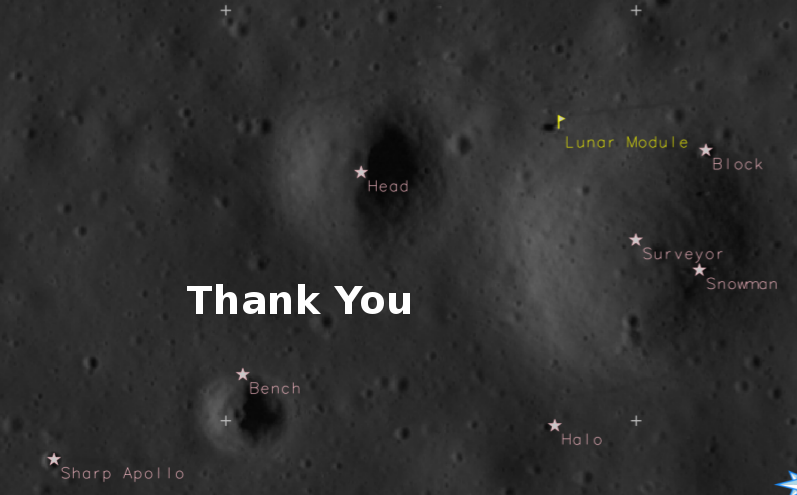
\includegraphics[width=12cm]{images/fig1_small}
\end{center}
\end{frame}

\end{document}
